%
%  Chapter:  3 - 135Pr Experimental Methods
%  Modified: 2/16/2015
%  Author:   James Till Matta
%
%%%%%%%%%%%%%%%%%%%%%%%%%%%%%%%%%%%%%%%%%%%%%%%%%%%%%%%%%%

\chapter{EXPERIMENTAL METHODS}
\label{chp:exp-pr}
Across experimental physics there is a common theme in the design of experiments. One part of this theme is finding a way to produce the system for study. Another part is designing the equipment to collect the signals required to interpret what the system is doing. In nuclear physics, the appropriate choice of reaction will create the desired system and the equipment for signal collection will depend on what is to be measured. This chapter will discuss the reaction, detectors, and techniques used in the examination of transverse wobbling in \pr{}.
\section{Heavy-ion Fusion-evaporation Reaction}
\label{sec:exp-pr-fus-evap}
Across nuclear physics there is a vast array of reactions used. Narrowing to in-beam \gr{} spectroscopy there are common ``workhorse'' reactions used. Of these workhorse reactions the heavy-ion fusion-evaporation reaction is frequently chosen for its selectivity in final products, producing relatively few species with large cross-section, and its creation of states with a large amount of angular momentum.\cite{beausang1996arrays}.
\subsection{Creation and Decay of the Compound Nucleus}
\label{ssec:exp-pr-fus-evap-cn}
The fusion-evaporation reaction proceeds by the formation of a highly excited compound nucleus, a mechanism first proposed by Neils Bohr\cite{bohr1936neutron}. While it is possible for a compound nucleus to be formed for beam energies below the coulomb barrier the probability is dramatically lower as the beam must quantum mechanically tunnel through the coulomb barrier. Therefore for heavy ion fusion to be experimentally feasible the center of momentum energy must exceed the height of the coulomb barrier. The coulomb barrier height can be estimated with

\begin{equation}
\label{eqn:chp3-cb_en}
E_{CB}=\frac{\alpha \hbar c Z_p Z_t}{1.16 fm (A_p^{1/3} + A_t^{1/3} + 2)}
\end{equation}

and the non-relativistic center of momentum energy is

\begin{equation}
\label{eqn:chp3-cmf_en}
E_{cm} = \frac{\mu}{A_{p}}E_{p}
\end{equation}

Here the subscripts $p$ and $t$ denote projectile and target respectively, $A$ is the mass number, $Z$ represents the nuclear charge, $\alpha{}$ is the fine structure constant, and $\mu = A_{p}A_{t}/(A_{p}+A_{t})$ is the system's reduced mass. After its formation the compound nucleus will have an excitation energy of

\begin{equation}
\label{eqn:chp3-cn_ex}
E_{ex} = Q + E_{cm}
\end{equation}

where $Q$ is the reaction's $Q$-value which is

\begin{equation}
\label{eqn:chp3-cn_form_qvalue}
Q = (M_t+M_p-M_{CN})c^2
\end{equation}

The compound nucleus will also carry an angular momentum ranging between $0 \hbar$ and $l_{max} \hbar$, corresponding to head on and peripheral collisions respectively. $l_{max}$ can be estimated classically as

\begin{equation}
\label{eqn:chp3-cn_lmax}
l_{max} = \frac{\sqrt{2\mu(E_{cm}-E_{CB})}}{4}(A^{1/3}_p + A^{1/3}_t)\hbar
\end{equation}

Following its formation a compound nucleus will be left in a state with high excitation energy. The two primary ways the compound nucleus rids itself of this excess energy are fission\cite{fastFission} or particle evaporation followed by \gr{} emission. A schematic of of a fusion-evaporation reaction is in Fig. \ref{fig:chp3-fus-evap-schem}.

\begin{figure}[h!]
	\centerline{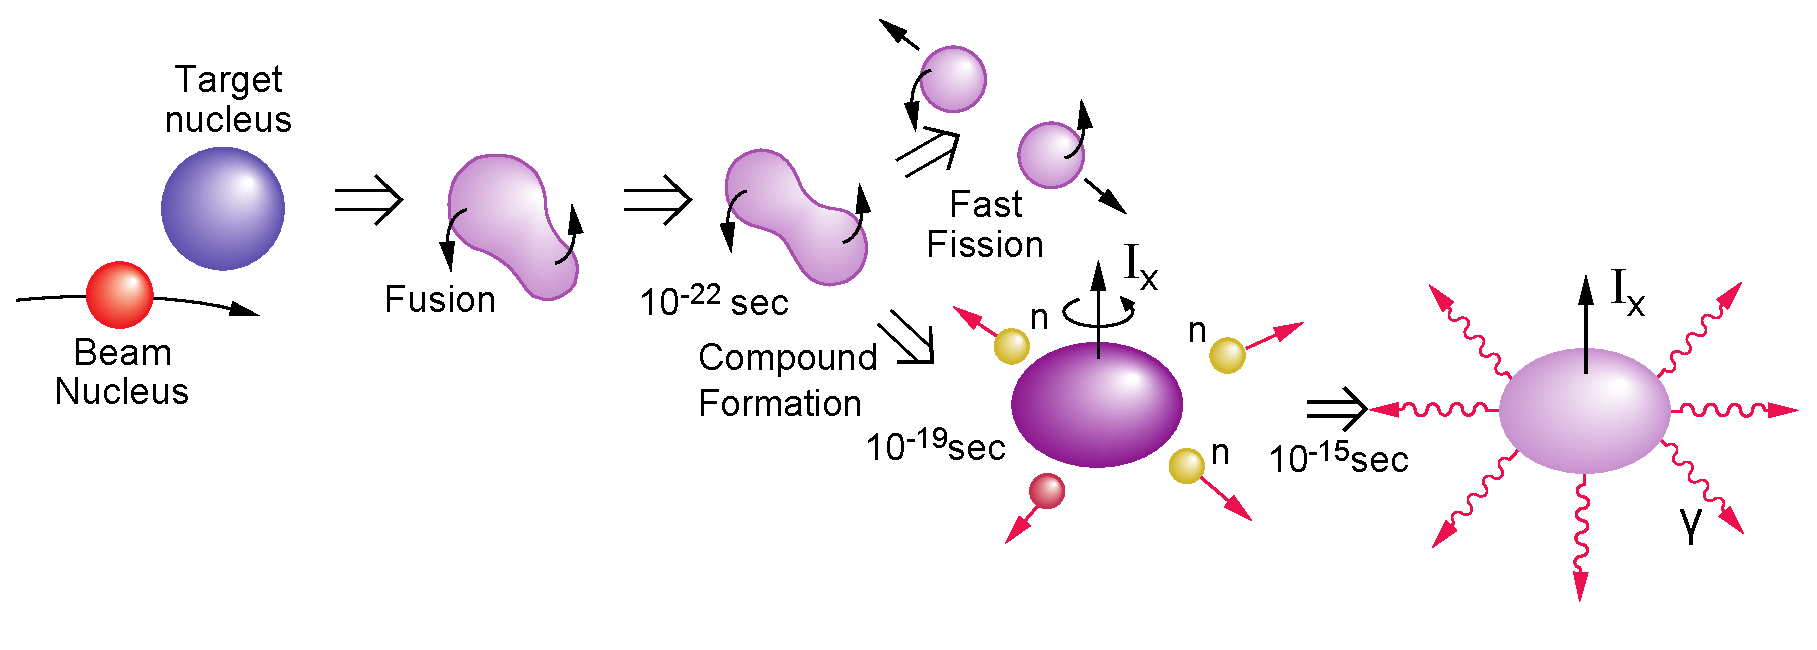
\includegraphics[width=\textwidth]{./img/c3/fusion_evaporation.pdf}}
	\caption{Schematic illustration of heavy-ion fusion-evaporation, adapted from Ref. \cite{gsBooklet}.}
	\label{fig:chp3-fus-evap-schem}
\end{figure}

The probability of the compound nucleus fissioning is governed by the height of the fission barrier relative to the its excitation energy. The height of the fission barrier is a function of the $A$ of the nucleus and is inversely proportional to the compound nucleus' angular momentum, as can be seen in Fig. \ref{fig:chp3-fission-barrier}. However, even the complete disappearance of the fission barrier does not guarantee fission as there are a few observed cases of spins above those required to reduce the barrier to zero\cite{hyperdef,hyperdef2}.

\begin{figure}[h!]
	\centerline{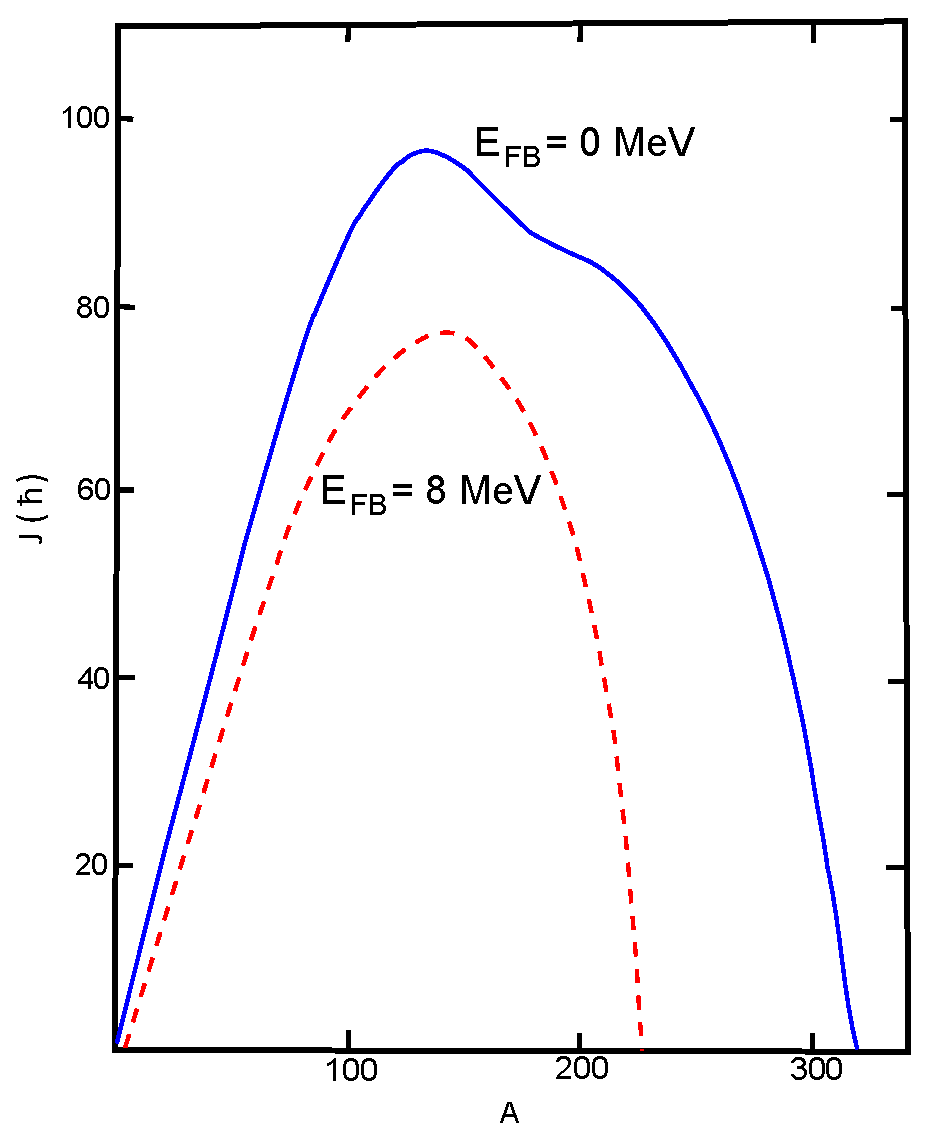
\includegraphics[height=0.3\textheight]{./img/c3/fission_barrier.eps}}
	\caption{Isocontours of angular momenta that yield fission barriers of $8MeV$ and $0MeV$ at various masses. Adapted from Ref. \cite{fissionBarrier2}.}
	\label{fig:chp3-fission-barrier}
\end{figure}

If the compound nucleus does not fission then it will instead evaporate particles. Particle evaporation is the emission of protons, neutrons, or alpha particles over or through an emission barrier. For charged particles this emission barrier is composed both of a centrifugal term which grows with increasing angular momentum and a coulomb term. For neutrons the emission barrier is solely the centrifugal barrier. In most cases neutron evaporation will be more probable, because charged particles encounter a higher barrier due to the coulomb term. The exception occurs for very neutron deficient nuclei where the reduction of proton separation energies make it possible for charged particle emission to compete with, or even dominate neutron emission. Each successive evaporated particle carries energy, but little angular momentum away from the nucleus until there is insufficient excitation energy for particles to penetrate the emission barrier and the nucleus is left in a state that is stable against particle emission. From this point on the nucleus must dissipate its excess angular momentum and excitation energy via \gr{} emission. A schematic of this can be seen in Fig. \ref{fig:chp3-emission-schematic}.

\begin{figure}[h!]
	\centerline{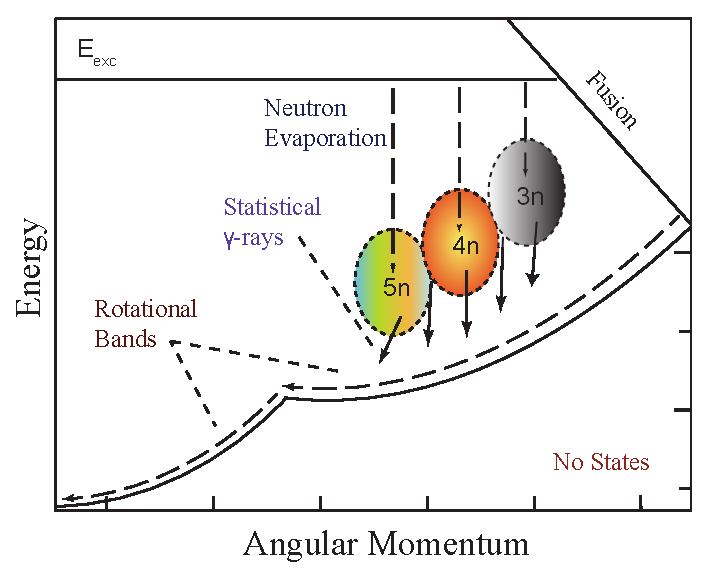
\includegraphics[height=0.3\textheight]{./img/c3/evaporation_chans.eps}}
	\caption{Schematic of the compound nuclear decay assuming that a rotational nucleus is being formed. Adapted from Ref. \cite{danielDissertation}.}
	\label{fig:chp3-emission-schematic}
\end{figure}

Initially the nucleus is in a state with such high level density that it decays by the emission of statistical \gr{}s\cite{cnCooling}. These statistical \gr{}s are almost purely dipole in nature and form a continuum as the notion of a discrete state is not a good one at such high level densities. As the nucleus approaches the yrast line (the states with the minimum excitation energy for a given angular momentum) the level density drops. This allows the emission sequences of discrete \gr{}s which feed the yrast line.

\subsection{Choice of Beam and Target}
\label{ssec:exp-pr-fus-evap-beam-target}
When choosing the beam and target for a fusion-evaporation several factors must be considered: What is the production cross-section of the desired residual nucleus? How clean is the production of the desired residual nucleus relative to the other residuals? What is the spin range to be studied? What is the availability of the isotopes to be used? What is the suitability of the material for beam production? While beam target combinations are usually chosen to maximize the cross-section for the desired residual, in some cases there are other channels open which will have large cross-sections themselves. In these cases the beam-target combination might be chosen to drastically lower the relative yield in competing channels at the cost of lowering the cross-section for the desired residual. For lower spins one usually chooses lighter projectiles. Eqn. \ref{eqn:chp3-cn_lmax} shows that it is possible to increase the angular momentum transfer with higher beam energies; however, this also increases the excitation energy of the compound nucleus, causing particle evaporation to be more probable. In the end, the decision is based on which combination yields the nucleus to be studied at the spins to be studied with the highest absolute and relative cross-sections possible.

Ref \cite{nucSpecAndReacPartC} gives the empirical estimate for $A_{CN}>100$ for obtaining the optimum beam energy for producing a specific residual nucleus in a (HI,xn) reaction, found below in Eqn. \ref{eqn:chp3-fe_peak_selection}.
\begin{equation}
\label{eqn:chp3-fe_peak_selection}
E_{pk}(x)=(-Q_{x} + \alpha{}x)(1+\frac{A_p}{A_t})
\end{equation}
Here $Q_x$ is the Q-value for the production of the residual nucleus given by:
\begin{equation}
\label{eqn:chp3-res_qvalue}
Q = (M_t+M_p-M_{res}-x M_n)c^2
\end{equation}
and $\alpha$ is $\sim6MeV$. The reaction will only have a reasonable cross-section if $E_{pk}(x)$ is greater than $E_{CB}$, which is the height of the coulomb barrier, given in Eqn. \ref{eqn:chp3-cb_en}. Computer codes that employ statistical models such as PACE4\cite{PACE4,PACE4_2} can now be used to calculate the cross-sections of products from these reactions allowing estimation of peak beam energies and optimal beam-target combinations. A plot of cross-sections yielded by calculations such as these can be found in Fig. \ref{fig:chp3-pace4-calc}.

\begin{figure}[h!]
	\centerline{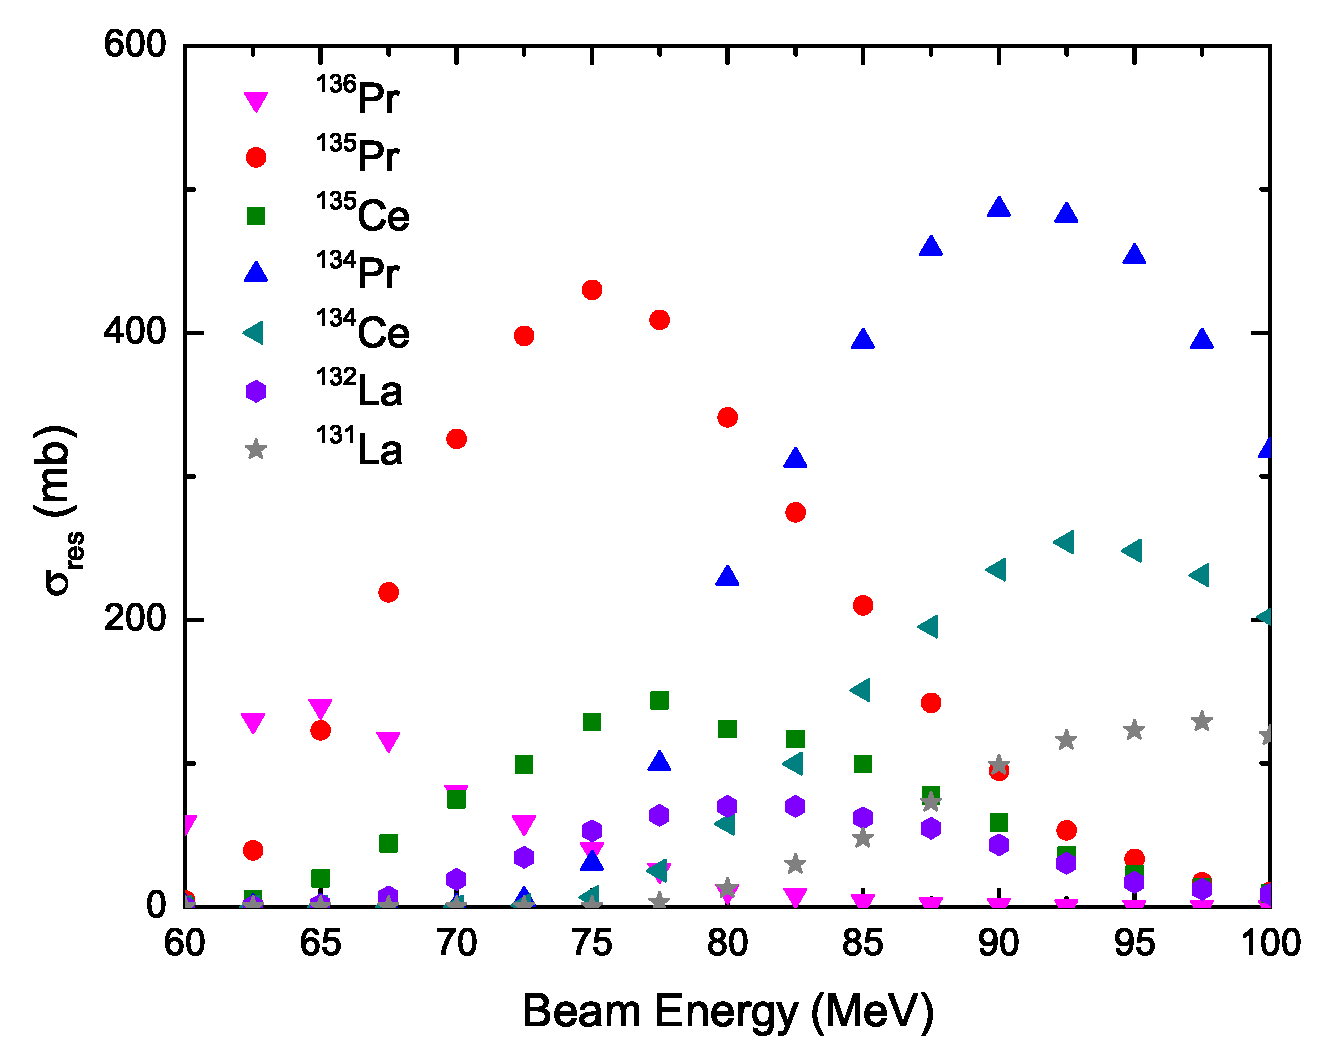
\includegraphics[width=\textwidth]{./img/c3/135Pr_calc_plot.eps}}
	\caption{Cross-sections of various residual nuclei for a $^{16}$O beam on $^{123}$Sb at a variety of beam energies as calculated by PACE4. As $^{139}$Pr is the compound nucleus produced all products that are not isotopes of Pr require the evaporation of a charged particle.}
	\label{fig:chp3-pace4-calc}
\end{figure}

\section{Gamma-ray Spectroscopy}
\label{sec:exp-pr-gamma-spec}
\subsection{Gamma-ray Interaction with Matter}
\label{ssec:exp-pr-gamma-spec-interactions}
As noted, the choice of equipment will vary with the signals to be collected to understand the system. One of the obvious signal choices for a residual nucleus at high spins is the \gr{}s it emits. Detection of gamma-rays is dependent on the \gr{} depositing energy in a detector which in turn depends on the interactions of electromagnetic radiation with matter. At the energies relevant to nuclear physics, $10keV<E_{\gamma}<15MeV$, there are three primary processes to be considered, photoelectric absorption, Compton scattering, and pair production. These three processes compete with each dominating in a different energy range.

In \emph{photoelectric absorption} the photon interacts with a bound electron in the detector material and is fully absorbed\cite{einstein-PE}. The total energy of the photon is then used to overcome the binding energy of the electron and to provide the electron with kinetic energy, giving $E_{e^-}=E_{\gamma}-E_b$. The electron then proceeds to lose energy as it passes through the detector material. In \gr{} spectra the full energy peak corresponds to the complete deposition of the primary photon's energy in the detector medium. For that to occur either the primary photon, or all the secondary photons (generated by the processes below), must undergo photoelectric absorption. As can be seen in Fig. \ref{fig:chp3-gamma-interactions} the photoelectric effect is dominant at low energies and the energy at which the photoelectric effect ceases to dominate increases with the Z of the material.

\begin{figure}[h!]
	\centerline{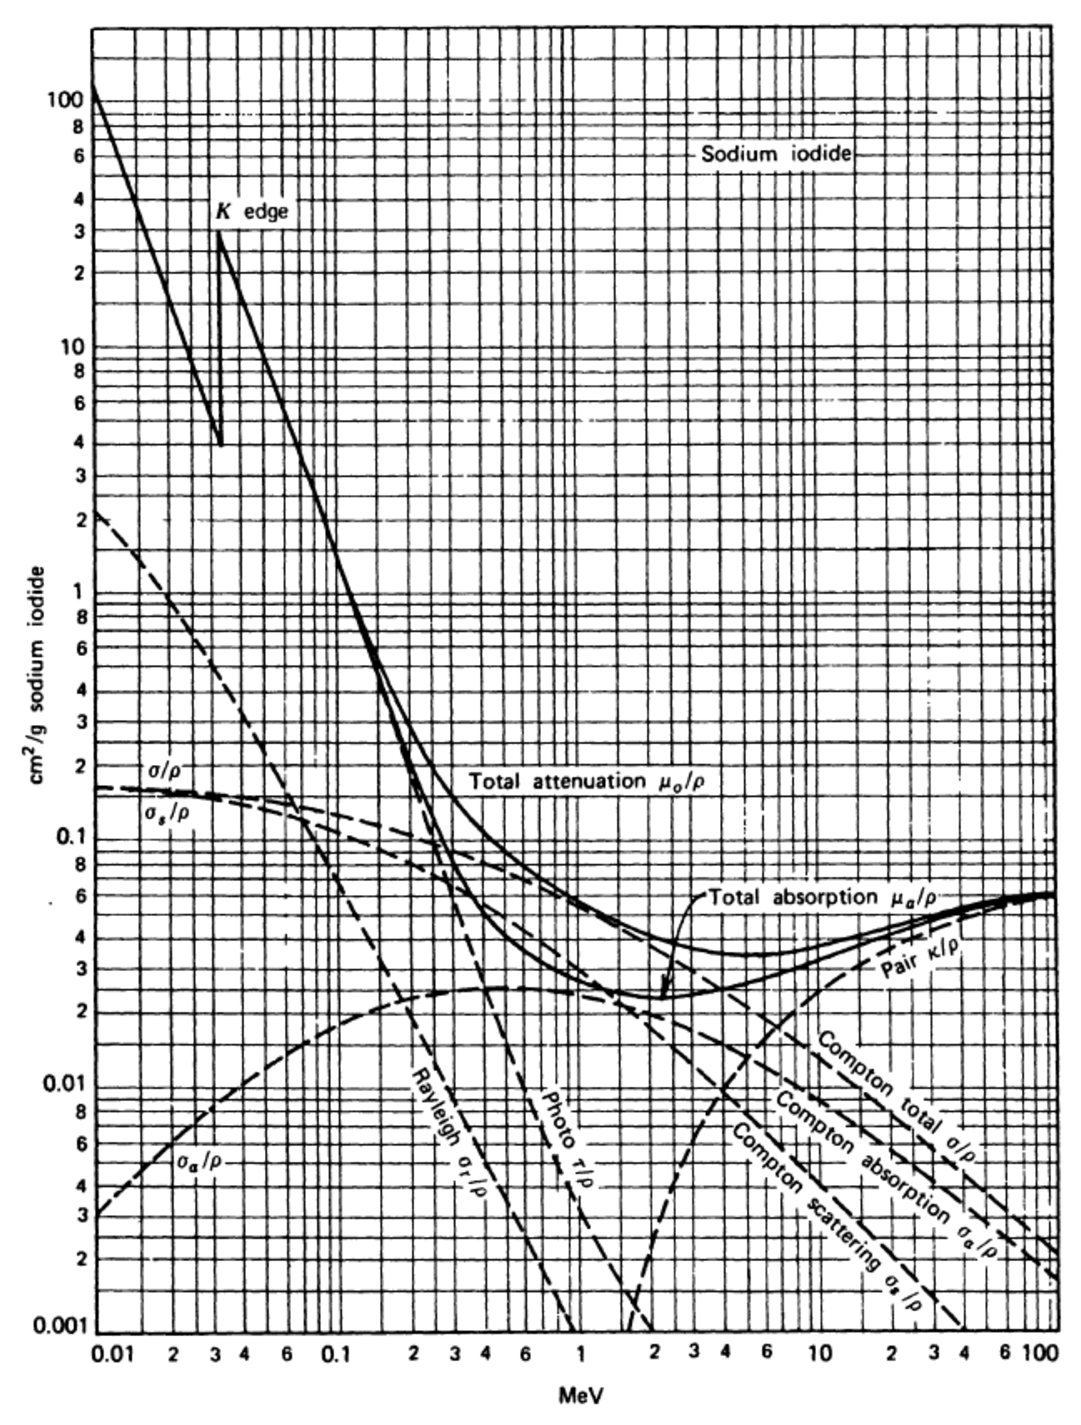
\includegraphics[height=0.5\textheight]{./img/c3/gamma_interactions_scan.eps}}
	\caption{Gamma-ray attenuation coefficients for various processes in NaI, adapted from Ref. \cite{knollBook}. Note the dominance of photoelectric absorption at lower energies, Compton scattering at intermediate energies, and pair production at high energies. While the slopes of these processes change from material to material, the trends remain the same.}
	\label{fig:chp3-gamma-interactions}
\end{figure}

In \emph{Compton scattering}, a \gr{} photon scatters from an electron in the material at some angle $\theta$ to its original direction\cite{Compton-PhysRev.21.483}. Due to conservation of momentum and energy, the energy transferred to the electron is precisely determined by $\theta$ and so the energy of the secondary photon can be written as: $E_{s}=E_{p}(1+\frac{E_{p}}{m_{e}c^2}(1-Cos\theta))^{-1}$ As above the electron then deposits its kinetic energy in the medium as it slows. However, unlike in the photoelectric effect, not all of the energy is deposited in the electron. After scattering, the secondary photon travels in its new direction and is free to interact again with probabilities dictated by its energy. Fig. \ref{fig:chp3-gamma-interactions} shows Compton scattering is the dominant effect at intermediate energies.

The final process to be considered is pair production. In pair production the photon enters the region of very strong electric field near the nucleus and its energy is converted into the mass and kinetic energy of an electron positron pair \cite{anderson-PhysRev.43.491,oppenheimer_PhysRev.44.53.2}. Since energy is conserved the photon must have energy of at least twice the rest mass of the electron, giving a threshold of $E_{\gamma}\geq1.022MeV$ for this interaction, any energy above this threshold is converted into kinetic energy shared between the two particles. After their production the electron and positron will both travel through the detector medium loosing energy as they travel. Once at rest the positron will annihilate with an electron, emitting two anti-parallel $511keV$ secondary photons. Fig. \ref{fig:chp3-gamma-interactions} shows the dominance of this interaction at high gamma energies; the energy at which pair production supersedes Compton scattering decreases with increasing Z of the material.

\subsection{High Purity Germanium (HPGe) Detectors}
\label{ssec:exp-pr-gamma-spec-hpge}
In detecting gamma-rays there are essentially 3 major classes of detector, scintillator, gas, and semiconductor detectors. In all cases the \gr{} enters the active volume of the detector and deposits energy by at least one of the processes mentioned above. The primary energetic electrons, produced directly by the interactions of the \gr{}, proceed to ionize or excite other electrons in the material. The secondary electrons are then detected in some manner. In scintillators the secondary electrons cause UV or visible light to be emitted and this is collected via photomultiplier tube, or similar device, to produce a voltage pulse. In gas and semiconductor detectors the charge of the secondary electrons (and their corresponding ions or holes) is collected directly, albeit via different mechanisms, to produce the voltage pulse.

It is desirable that \gr{} detectors have both good detection efficiency and energy resolution. Current \gr{} detectors are unable to satisfy both goals. It is necessary to decide which parameter is more important. For high spin experiments where the spectrum is dense with peaks, the energy resolution is the top priority since broad peaks would be indistinguishable from each other. Of the available detectors, semiconductor detectors, particularly High Purity Germanium (HPGe) detectors offer the best energy resolution.

Semiconductor detectors are reversed bias diodes with either a p-n or a p-i-n junction. At the boundary between the types of materials there is a so called contact potential. This potential gives rise to an electric field which causes the migration of charges between the two materials until there is an area bridging the boundary called the depletion zone. In this zone there is an electric field which gives rise to a potential that counters the contact potential. By applying reverse bias to the diode the contact potential is effectively increased causing the depletion zone to expand (schematic in Fig. \ref{fig:chp3-pn_diode}). This is desirable because the depletion zone is the only region of the semiconductor where an electric field will exist. This means that electron hole pairs formed within it are swept away from each other for collection before they can recombine. In contrast, electron hole pairs formed outside the depletion zone are not pulled away from each other and thus recombine, preventing their collection. Due to this, the depletion zone of the detector is the region that is active. That is to say that the passage of ionizing radiation through that region is detectable because the electron hole pairs produced are collected.

\begin{figure}[h!]
	\centerline{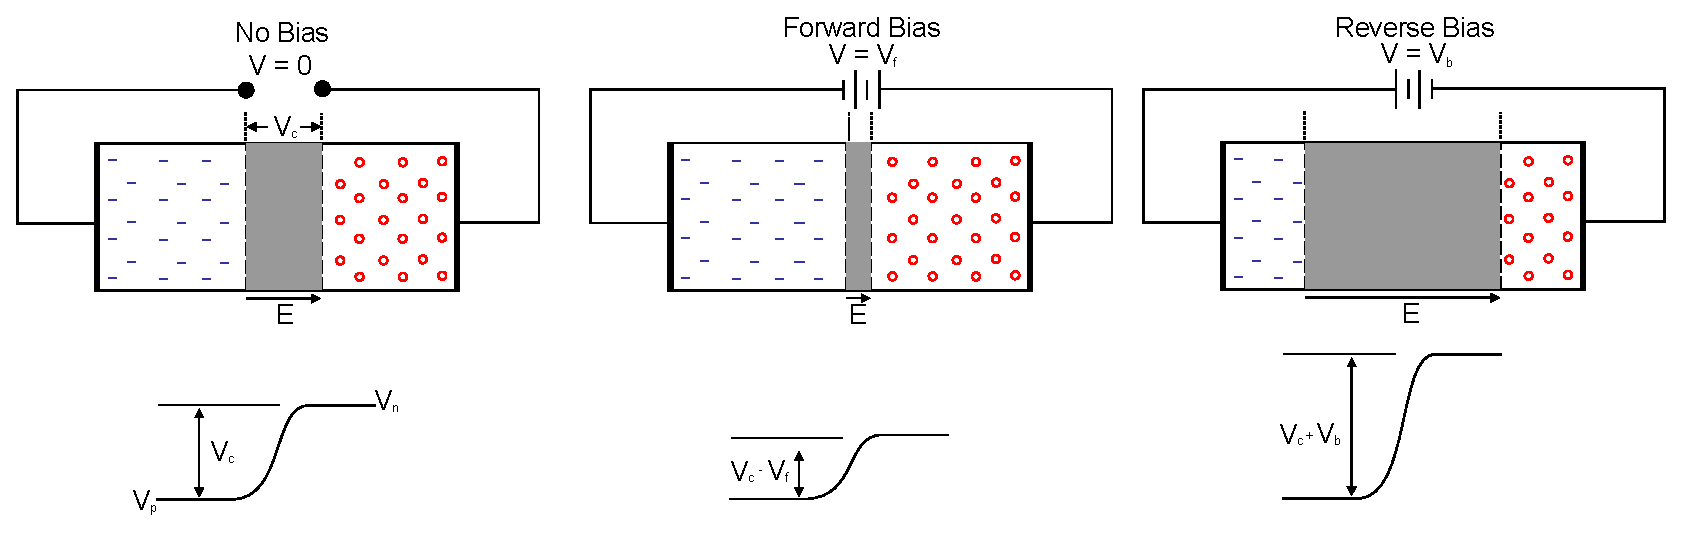
\includegraphics[width=\textwidth]{./img/c3/pn-diode.eps}}
	\caption{Above: Diagrammatic view of the depletion zone's with varying bias voltage. Below: Voltage difference across the depletion zone for each bias voltage shown above.}
	\label{fig:chp3-pn_diode}
\end{figure}

The higher the purity of the semiconductor, the higher the reverse bias voltage that can be applied without reaching the breakdown of the semiconductor (usually a catastrophic event). In HPGe detectors the purity is sufficiently high that the whole crystal of Ge can be depleted yielding a very large active region, an advantage for \gr{}s given their low interaction probabilities compared to charged particles. When a gamma interacts in an HPGe detector it produces at least one high energy secondary electron or positron (more if there are multiple interactions). These secondary electrons lose energy quickly as they pass through the detector, leaving a trail of electron hole pairs in their wake. The electrons and holes are then swept to their respective contacts by the applied potential and collected.

A detector's resolution is defined as the FWHM for a given peak. The intrinsic resolution of a semiconductor detector stems from statistical fluctuations in how many electrons and holes are collected at the terminals. These fluctuations arise from simple counting statistics; their form can be described by:
\begin{equation}
\label{eqn:chp3-hpge-res-est} 
\Delta{}E_{in} \propto \frac{E_{\gamma}}{\sqrt{N}}
\end{equation}
Where N is the number of charge carriers produced and is approximately $E_{\gamma}/\epsilon$ where $\epsilon$ is the average energy to make an electron hole pair ($2.96eV$ for Ge). In a more precise examination the intrinsic component of the FWHM is:
\begin{equation}
\label{eqn:chp3-hpge-in-res} 
\begin{split}
\Delta{}E_{in}(E) & = 2\sqrt{2 ln(2)}\frac{\sqrt{F E_{\gamma{}}/\epsilon{}}}{E_{\gamma{}}/\epsilon{}}E_{\gamma{}}\\
       & = 2.355\sqrt{F\epsilon{}E_{\gamma{}}}
\end{split}
\end{equation}
Here $F$ is the Fano factor. This value, intrinsic to the detector material, ranges across $(0,1]$ and takes into account energy loss mechanisms available to the secondary electron(s) that do not generate electron hole pairs. A more thorough explanation is available in Refs. \cite{knollBook,fano_factor1}.

Unfortunately, the detector's intrinsic resolution is not the only contributor to the detector's resolution. There are also contributions from such sources as electronic noise, charge carrier collection / trapping, and Doppler broadening. If it is assumed that these components are independent and normally distributed, the actual resolution is:
\begin{equation}
\label{eqn:chp3-hpge-res} 
\Delta{}E_{T}^2 = \Delta{}E_{in}^2 + \Delta{}E_{E}^2 + \Delta{}E_{C/T}^2 + \Delta{}E_{D}^2
\end{equation}
Where $\Delta{}E_{E}$ is the electronic noise contribution, $\Delta{}E_{C/T}$ is the charge collection / trapping term, and $\Delta{}E_{D}$ is the Doppler broadening term. Ref. \cite{trappingResolution} gives the FWHM forms of the noise and collection / trapping terms as:
\begin{equation}
\label{eqn:chp3-hpge-res-noise} 
\Delta{}E_{E} = N_{1/2}
\end{equation}
\begin{equation}
\label{eqn:chp3-hpge-res-ct} 
\Delta{}E_{C/T} = 2.355\sqrt{\epsilon{} K E_{\gamma{}} [1-\eta{}(\vec{r})]}
\end{equation}
Where $N_{1/2}$ is the FWHM of the electronic noise, $K$ is a constant of a given detector, and $\eta{}(\vec{r})$ is the total charge collection efficiency of electrons and holes of the detector as a function of the interaction site's position.

\begin{figure}
	\centerline{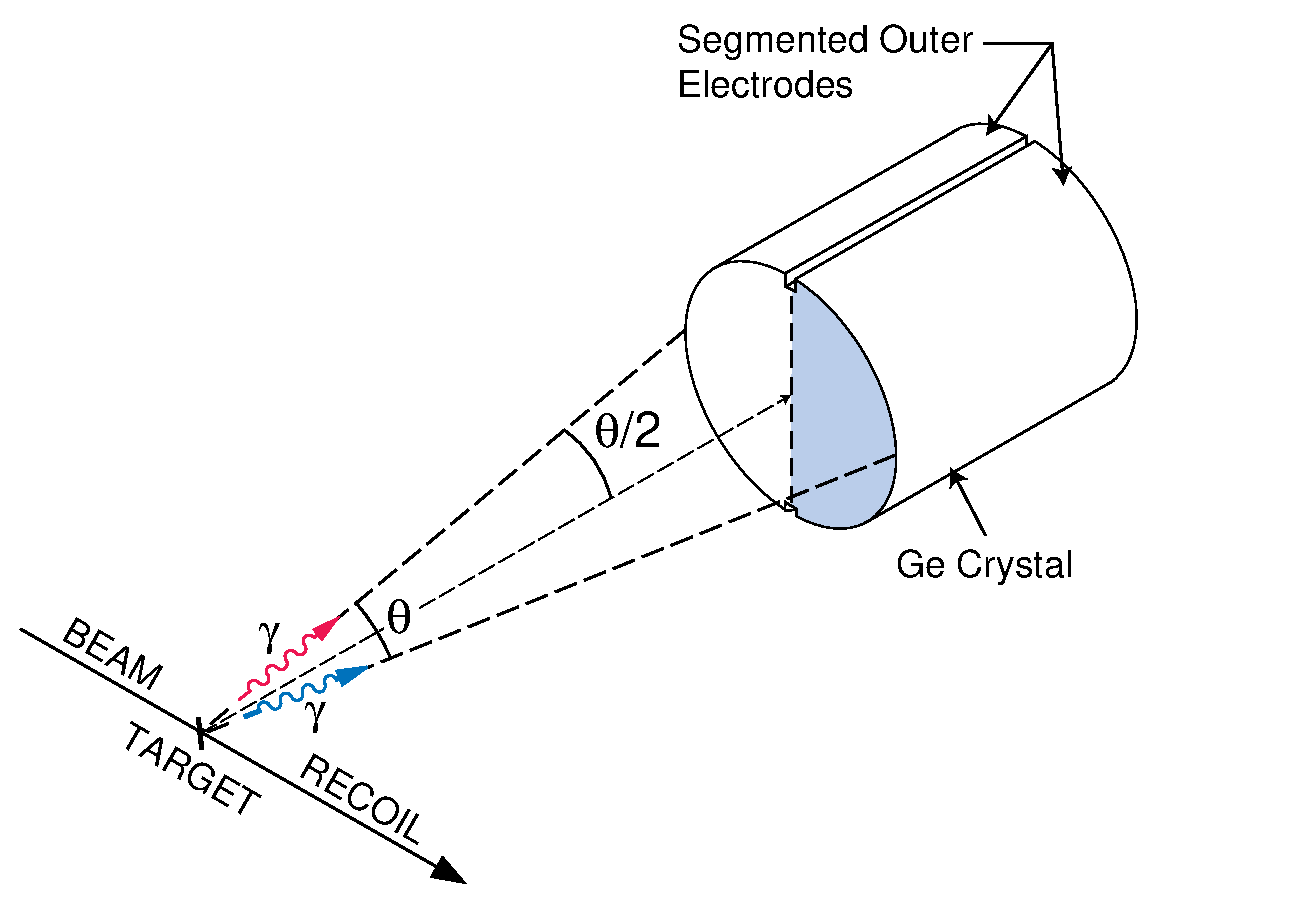
\includegraphics[height=0.3\textheight]{./img/c3/split_contact.eps}}
	\caption{Diagram showing the uncertainty inherent in the \gr{}'s angle of emission, and Gammasphere's segmented electrode scheme to reduce this.}
	\label{fig:chp3-doppler-split-contact}
\end{figure}

The final term, $\Delta{}E_{D}$, of this equation comes from uncertainty in the angle at which the gamma ray was emitted from the recoiling nucleus due to the detectors finite size (shown in Fig. \ref{fig:chp3-doppler-split-contact}). The shift in gamma energy due to the nuclear recoil is:
\begin{equation}
\label{eqn:chp3-doppler_formula} 
E_{o} = E_{e}\frac{\sqrt{1+\beta{}Cos(\theta)}}{\sqrt{1-\beta{}Cos(\theta)}}
\end{equation}
here, the subscripts o and e refer to observed and emitted, $\beta$ is the speed of the recoiling nucleus divided by $c$ and theta is the angle between the nucleus' line of a flight and the emitted \gr{}. If the detector has an angular acceptance of $\theta{}_{0}-\delta{}\theta{}\leq{}\theta{}\leq{}\theta{}_{0}+\delta{}\theta{}$ with $\theta{}_{0}$ the central angle of the detector then the leading order term of the Doppler broadening contribution to the resolution is:
\begin{equation}
\label{eqn:chp3-res-doppler-term} 
\Delta{}E_{D} = 2\beta{}Sin(\theta{})Sin(\delta{}\theta{})E_{\gamma}
\end{equation}
There are three strategies to combat this term. The first is geometrical. By increasing the granularity of the array, either by using more and smaller detectors or by using more detectors at a longer distance from the source. This in turn would shrink the opening angle of detectors and therefore reduce the Doppler broadening. The second method is electrical in nature, by segmenting the outer contact of the detector, even roughly, the location of the interaction within the detector can be determined. This effectively reduces the opening angle. Gammasphere uses this strategy as shown in Fig. \ref{fig:chp3-doppler-split-contact}. The split outer contact allows the reduction of the effective opening angle, $2\delta{}\theta{}$, from $14.9^{\circ}$ to $7.45^{\circ}$ \cite{TheGS}. The third method involves a physical segmentation of the detector by having multiple crystals in close proximity within the same cryostat. This combination produces a detector that has a volume equal to the sum of the individual crystal volumes. However, despite this large volume, the opening angle of the individual crystals is the opening angle to consider for the Doppler broadening. Thus a physically segmented detector can give you a smaller Doppler broadening than an unsegmented detector of the same volume.  Clover and cluster detectors\cite{cloverDet,clusterDetector} are examples of this strategy.

\subsection{Escape Suppression with BGO Detectors}
\label{ssec:exp-pr-gamma-spec-escape-supress}
The primary contribution to the background in \gr{} spectroscopy is the incomplete deposition of energy in the detector. Two of the mechanisms discussed in section \ref{ssec:exp-pr-gamma-spec-interactions} can lead to this. Compton scattering will result in incomplete energy deposition when the secondary photon yielded by the process escapes the HPGe crystal without depositing the rest of its energy. This mode results in a smooth background from the maximum energy transferable to an electron in the process down to zero energy. Pair production will yield incomplete energy deposition when one or both of the photons from the annihilation of the positron escape the detector. This mode results in 2 new peaks forming, the first $511keV$ below the photopeak, corresponding to one annihilation photon escaping, and a second $1022keV$ below the photopeak, corresponding to both escaping.
\begin{figure}[h!]
	\centerline{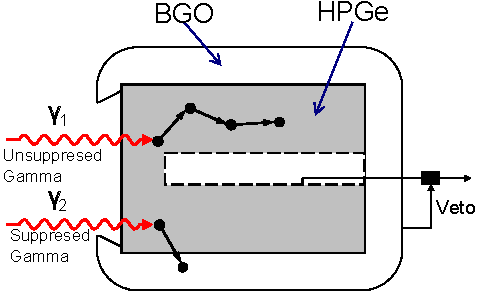
\includegraphics[height=0.25\textheight]{./img/c3/BGO_schematic.pdf}}
	\caption{Schematic of BGO escape suppression around an HPGE crystal.}
	\label{fig:chp3-supression-schematic}
\end{figure}

To ameliorate this the principal detector is surrounded by a secondary detector and the electronics are set to be in anti-coincidence (see Fig. \ref{fig:chp3-supression-schematic} for a schematic). If both detectors had energy deposited, the event is discarded. In practical application, the second detector must be highly efficient at detecting gammas to minimize its size. Given this constraint, the scintillator Bismuth Germanate (BGO) is an excellent choice for escape suppression. While BGO's energy resolution is quite poor, it has excellent timing characteristics, quite high density, and is made of fairly high $Z$ materials. The latter two facts give it the desired high detection efficiency (substantially higher than the HPGe it is shielding). Improvements up to a factor of $2.48$ in the peak-to-total ratio (P/T) can be seen for some designs. A bare HPGE detector having a (P/T) of $0.270\pm0.002$ has been shown to improve to $0.669\pm0.002$\cite{GSComptonSuppression} with an escape suppression shield around the sides and part of the back (some space needs to be left for cables to exit the HPGe.) Example spectra showing this improvement can be seen in Fig. \ref{fig:chp3-supression-improvement}.

\begin{figure}[h!]
	\centerline{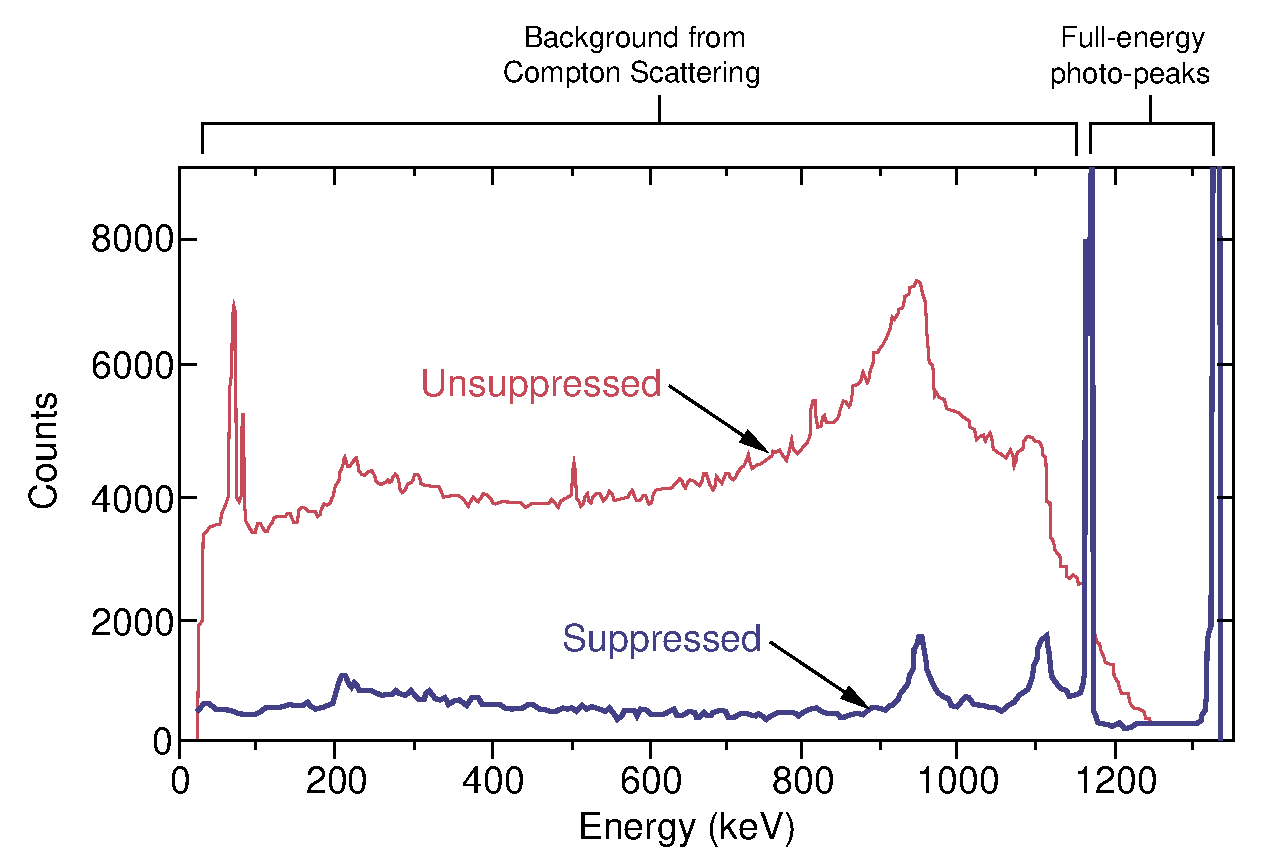
\includegraphics[height=0.25\textheight]{./img/c3/suppressed_spectra.eps}}
	\caption{Superimposed spectra of an escape suppressed and unsuppressed detector. Adapted from Ref.\cite{gsBooklet}}
	\label{fig:chp3-supression-improvement}
\end{figure}

\subsection{The Gammasphere Detector Array}
\label{ssec:exp-pr-gamma-gammasphere}
Gammasphere (partially pictured in Fig. \ref{fig:chp3-gs-hemisphere}) is an array of $110$ escape suppressed HPGe detectors arranged in a sphere around a target. A cross sectional view of part of the array can be seen in Fig. \ref{fig:chp3-gs_det_schem}. The BGO shields are arranged in hexagonal shapes around each detector plus a backplug covering the majority the back of the detector. Gammasphere's spherical geometry is comprised of 17 rings of detectors, each ring at a distinct angle to the beam axis. Using a scheme called honeycomb suppression, Gammasphere has a total efficiency of $~0.09$ at $1MeV$ and a singles P/T of $0.69$.

\begin{figure}[h]
	\centerline{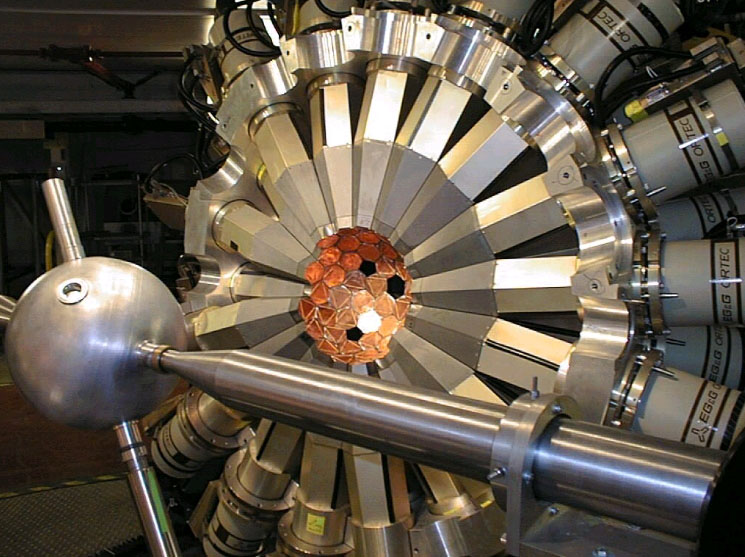
\includegraphics[height=0.3\textheight]{./img/c3/gammasphere_hemi.jpg}}
	\caption{View of scattering chamber and interior of one of Gammasphere's hemispheres pulled back from the chamber. The hexagonal copper foils are x-ray absorbers.}
	\label{fig:chp3-gs-hemisphere}
\end{figure}

\begin{table}[ht!]
\caption{GAMMASPHERE FEATURE SUMMARY\label{tbl:gs-summary}}
\begin{center}
\begin{tabular}{|c|c|}
\toprule
No. Detectors             & 110 \\ 
No. Segmented Detectors   & 70 \\ 
HPGe Detector Size        & $7.1 cm$ (D) $\times$ $8.22 cm$ (L) \\
Detector Volume           & $312.8 cm^3$\\
Target to HPGe Front      & $24.6 cm$\\ 
Total HPGE Solid Angle    & $0.46 \times 4\pi$\\ 
Total Peak Efficiency     & $0.094$ at $1.3 MeV$\\ 
Singles P/T               & $0.6$ at $1.3 MeV$ \\ 
Energy Resolution (MeV)   & $2.1keV$ at $1.3 MeV$ \\ 
\bottomrule
\end{tabular}
\end{center}
\end{table}

\begin{figure}[h]
	\centerline{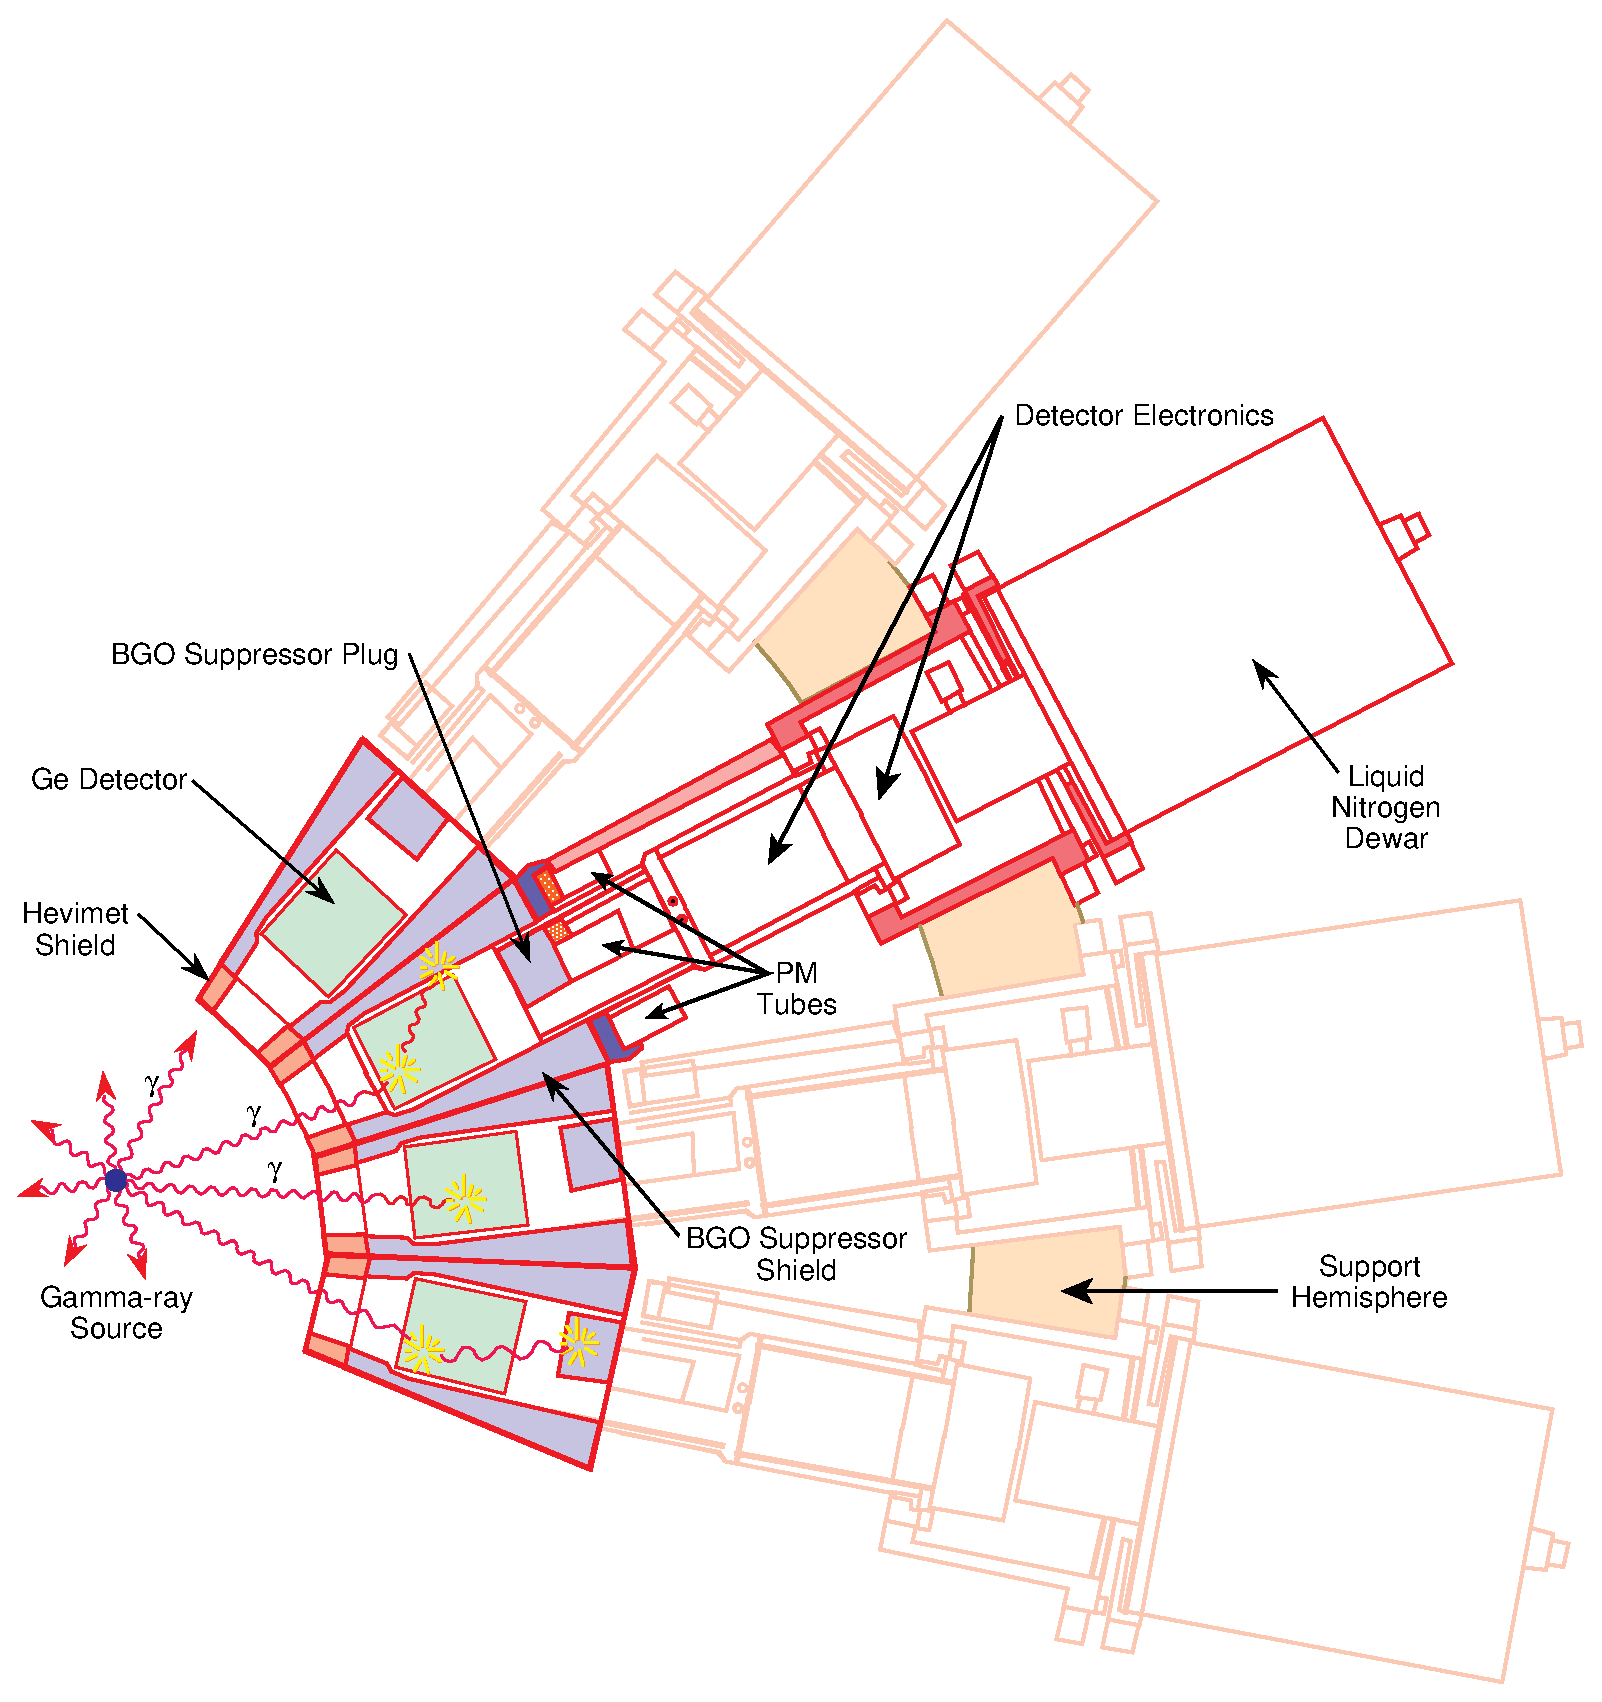
\includegraphics[height=0.3\textheight]{./img/c3/gammasphere_detector.eps}}
	\caption{Cross-section schematic of part of Gammasphere. Adapted from Ref.\cite{gsBooklet}}
	\label{fig:chp3-gs_det_schem}
\end{figure}

Honeycomb suppression is an escape suppression scheme that uses the BGO shields of adjacent detector modules to effectively double the thickness of a detector's shields. As seen in Fig. \ref{fig:chp3-gs_det_schem} almost every module will have additional modules immediately adjacent to it. If the HPGe detector for a given module do not register energy deposition the 6 side segments of its BGO shield are used to double the thickness of the shields they are adjacent to. Without this measure the singles P/T is $\sim0.62$; using honeycomb suppression improves this to $\sim0.69$ though it reduces the total efficiency at 1.332MeV from $\sim0.095$ to $\sim0.089$\cite{TheGS}. Table \ref{tbl:gs-summary} contains a brief summary of Gammasphere's features drawn from Refs. \cite{TheGS,SimulatedResGS,GSComptonSuppression,largeArrays}.

As mentioned in section \ref{ssec:exp-pr-gamma-spec-hpge} some of Gammasphere's detectors have a split outer electrode to reduce the effective half angle. Detector positions can be found in table \ref{tbl:app1-gs-rings} and table \ref{tbl:app1-gs-detectors} in appendix \ref{app:gs-rings-and-detectors}. Gammasphere's high granularity, good energy resolution, and efficiency make it a boon for high \gr{} multiplicity coincidence measurements.

\subsection{Indian National Gamma Array (INGA)}
\label{ssec:exp-pr-gamma-spec-inga}
The Indian National Gamma Array (pictured in Fig. \ref{fig:chp3-INGA}) is an array of 24 escape suppressed HPGe clover detectors\cite{ingaAtIUAC}. Since INGA utilizes clover detectors it is sensitive to the polarization of \gr{}s emitted from nuclei in aligned states\cite{cloverDet}. Additionally, the use of clover detectors make the array more efficient for high energy \gr{} when using add back mode to sum the energies deposited in each of the individual crystals.

\begin{figure}[h!]
	\centerline{\includegraphics[height=0.25\textheight]{./img/c3/INGA.JPG}}
	\caption{Exterior view of INGA.}
	\label{fig:chp3-INGA}
\end{figure}

INGA's current incarnation utilizes a digital data acquisition system (DAQ) that allows it to run in a triggerless mode producing timestamped gamma data from a $10ns$ clock\cite{IngaDigitalDAQ}. Digital data acquisition systems, because they digitize the preamp signal directly, can operate at higher counting rates than analog because they do not require multiple microseconds of signal shaping time. The downside of this mode is that coincidences are not prebuilt by the DAQ and instead need to be constructed by moving a sliding window of the desired coincidence time across the timeline of events and selecting sets of gammas that occur within that window. A final advantage of the time stamped events is that isomers can have their lifetime measured using time differences between \gr{}s as seen in Fig. \ref{fig:chp3-INGA-isomer}.

\begin{figure}[h!]
	\centerline{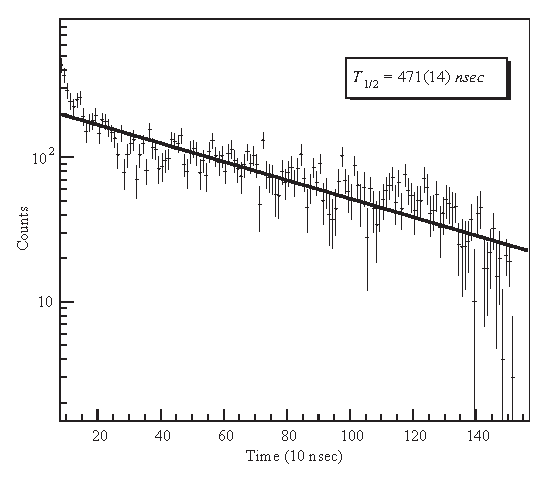
\includegraphics[height=0.35\textheight]{./img/c3/INGA_isomer.eps}}
	\caption{Example isomer timing spectrum for INGA. From Ref. \cite{IngaDigitalDAQ}.}
	\label{fig:chp3-INGA-isomer}
\end{figure}

Using its digital DAQ and add-back on the clover crystals, INGA achieves a total efficiency of $\sim0.05$ and P/T of $0.4$ at $\sim1.33MeV$. Table \ref{tbl:inga-summary} contains summary of INGA's features. INGA's sensitivity to polarization, efficiency, and granularity make it a good system for intermediate \gr{} multiplicity coincidence measurements, reaching its best efficiency at 2- to 3-fold events.

\begin{table}[ht!]
\caption{INGA FEATURE SUMMARY\label{tbl:inga-summary}}
\begin{center}
\begin{tabular}{|c|c|}
\hline
\hline
No. Clover Detectors      & 24\\ 
No. Single Crystals       & 96\\ 
Single Crystal Size       & $5 cm$ (D) $\times$ $7 cm$ (L) \\
Single Crystal Volume     & $117.5 cm^3$\\
Target to HPGe Front      & $24 cm$\\ 
Total HPGE Solid Angle    & $0.25 \times 4\pi$\\ 
Total Peak Efficiency     & $0.05$ at $\sim1.0 MeV$\\ 
Singles P/T               & $0.40$ at $1.3 MeV$ \\ 
Energy Resolution (MeV)   & $2.2keV$ at $1.3 MeV$ \\ 
\hline 
\hline 
\end{tabular}
\end{center}
\end{table}

\section{Experimental Details}
\label{sec:exp-pr-details}
The work on \pr{} presented in this dissertation was performed at two different facilities, the ATLAS (Argonne Tandem Linear Accelerator System) facility with the Gammasphere detector system and the TIFR-BARC Pelletron LINAC with the INGA detector system. At both facilities the $^{16}O(^{123}Sb,4n)^{135}Pr$ reaction was used. As mentioned in section \ref{sec:exp-pr-fus-evap} the choice of beam and target affects both the most probable channel, the excitation energy, and the maximum angular momentum of the compound (and residual) nucleus. In previous in-beam \gr{} spectroscopy literature the following heavy ion fusion-evaporation reactions have been used to reach yield the \pr{} residual nucleus: $^{120}Sn(^{19}F @ 91MeV,4n)^{135}Pr$\cite{Semkow135Pr}, $^{123}Sb(^{16}O @ 76MeV,4n)^{135}Pr$\cite{135PrLifetimes}, and  $^{116}Cd(^{23}Na @ 115MeV,4n)^{135}Pr$\cite{EPaul135Pr}. The $^{16}$O and $^{123}$Sb projectile-target combination was chosen for its lighter projectile to optimize for population of states further from the yrast line.

\subsection{ATLAS/Gammasphere}
\label{ssec:exp-pr-details-gs}
ATLAS is located at the Physics Division at Argonne National Laboratory in Argonne, Illinois, USA. ATLAS is the world's first superconducting ac linear accelerator (linac) for projectiles heavier than an electron. It consists of 3 sections. The first of these sections is the injector accelerator which can be either a 9 Megavolt (MV) tandem Van de Graff accelerator or an electron cyclotron resonance (ECR) ion source coupled to a 12 MV low velocity LINAC (``PII'', Positive Ion Injector). The beam from the chosen injector is sent the 20 MV ``booster'' linac and finally to the 20 MV ``ATLAS'' linac. This system produces pulsed beams with spot diameter $\leq1mm$, pulse length $\leq500ps$, and interval $82ns$ which range across all elements from hydrogen to uranium with energies of $7-17MeV$ per nucleon ($/\mu{}$.)

The Gammasphere detector system was used in the FMA (Fragment Mass Analyzer) position though the FMA itself was not used. This configuration requires that the first ring of detectors at $\theta{}=17.27465^{\circ}$ be removed from the array due to a lack of space. Additionally several other detectors were removed from the array due to various issues. A complete listing of the detector numbers missing from the array is presented in Table \ref{tbl:app1-gs-missing-det} in Appendix \ref{app:gs-rings-and-detectors}.

Multiple self supporting $^{123}$Sb targets were prepared for the experiment using 98.28\% enriched powder from ISOFLEX USA (PO Box 29475, San Francisco, CA 94129 USA)\cite{sbTargets}. Due to the low thermal conductivity ($0.243W/cm/K$ at $300K$\cite{thermalCond}) and high vapor pressure\cite{sbPartialP,sbTargets} of Sb a thin layer ($14\mu{}g/cm^2$) of Al was deposited on the front surface of several of the targets created. This served the dual purpose of helping to dissipate the heat deposited in the target by the beam and of inhibiting sputtering of the target. Of the targets that had the Al layer, two ($630\mu{}g/cm^2$ and $634\mu{}g/cm^2$) were placed on the target ladder for Gammasphere (as well as a beam viewer). An oxygen beam of $3pnA$ at $81.2MeV$ was then impinged on the $634\mu{}g/cm^2$ target (the other target served as an unnecessary backup in case of failure of the primary target.) To further reduce the risk of evaporating a hole in the target, the beam was wobbled by placing a sinusoidal voltage on vertically and horizontally positioned plates upstream of the target. The amplitudes were $1.0V$ for the $\uvec{x}$-axis and $1.1V$ for the $\uvec{y}$-axis.

\subsection{TIFR - BARC Pelletron LINAC / INGA}
\label{ssec:exp-pr-details-inga}
The TIFR-BARC pelletron linac is located at the Tata Institute of Fundamental Research (TIFR), Mumbai, India. It is a collaborative project between TIFR and the Bhabha Atomic Research Centre (BARC) and is the first superconducting heavy ion accelerator in India. The first section of the system is a 14MV tandem Van de Graaf accelerator. The beam emitted from the pelletron is then bunched and injected into a linac yielding beam pulses with a width of $\sim{}600ps$ ranging across most of the elements from hydrogen to chlorine at $5-10MeV/\mu{}$.

The INGA detector system was used in its standard position at the facility; however, a few detectors were not present due to various problems. A summary of the electronics connections and detectors is in Table \ref{tbl:app2-inga-detectors}.

The two self supporting targets used in the Gammasphere experiment were given thick gold backings of $20.3mg/cm^2$ for the $630\mu{}g/cm^2$ target and $22.8mg/cm^2$ for the $634\mu{}g/cm^2$\cite{sbTargets}. This served several purposes: first and foremost the thick backing helped the delicate Sb targets survive transport to India. Second, the backing would allow a doppler shift attenuation measurement to determine lifetimes. (this unfortunately proved impossible.) Finally, the thick gold backing allowed heat deposited in the target by the beam to be easily dissipated, negating the need for a beam wobbling system.

\section{Data Processing}
\label{sec:exp-pr-data-proc}
 As stated earlier, this work was performed at two facilities. In the experiment using Gammasphere $\sim{}185$Gb of data spread across $104$ files were collected. The data set was comprised of $3.57\times{}10^9$ three- and higher-fold events with the distribution across folds shown in Fig. \ref{fig:chp3-gs_event_pattern}. While the system was set to not trigger for less than three-fold events, lower events still make it through due to honeycomb suppression. Because honeycomb suppression is applied after the system has triggered it effectively removes gammas from an event, reducing its fold, even to below the threshold set in the trigger system. The data from this experiment were used for the reconstruction of the level scheme and extraction of angular distributions and DCO ratios.
 
\begin{figure}[h!]
	\centerline{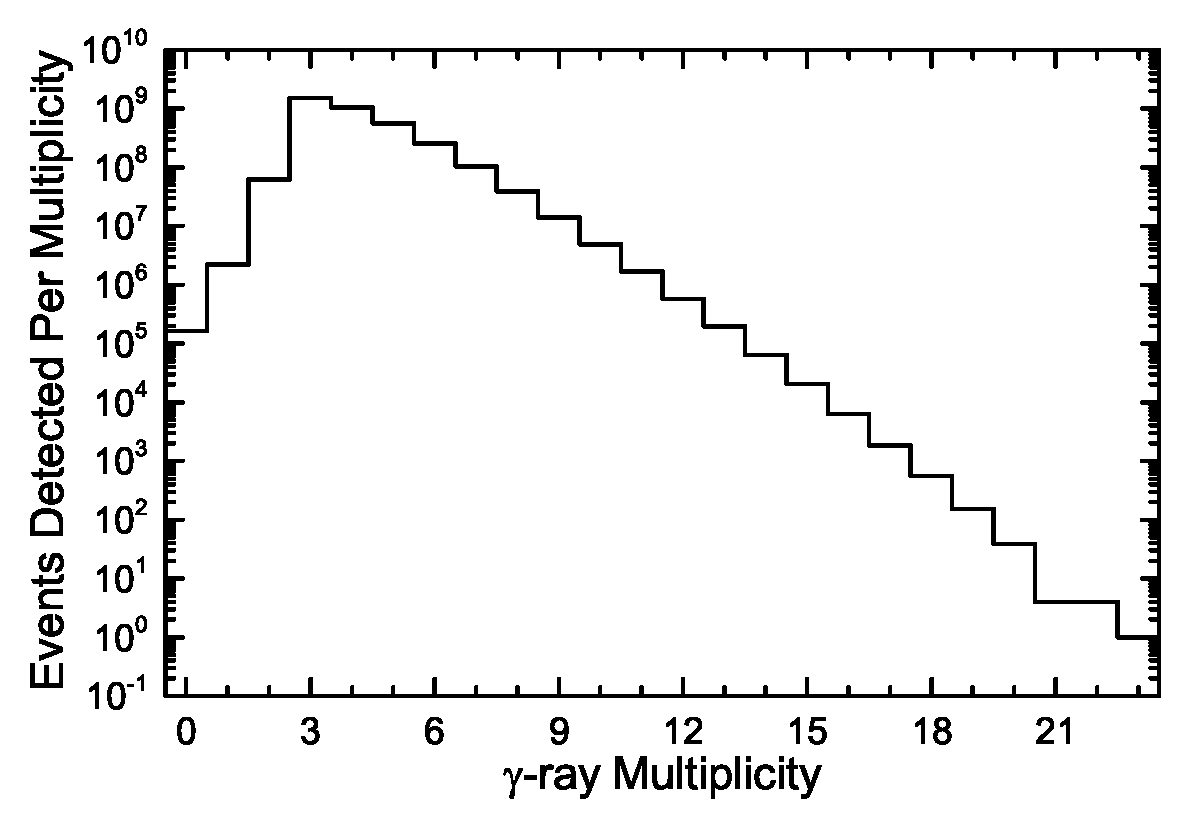
\includegraphics[height=0.25\textheight]{./img/c3/gs_event_plot.eps}}
	\caption{Histogram of the number of events in each multiplicity for the experiment at Gammasphere.}
	\label{fig:chp3-gs_event_pattern}
\end{figure}
 
In the experiment utilizing INGA $\sim{}550$Gb of data spread across $\sim800$ files were collected. As INGA was run in a triggerless mode each module of electronics output timestamped events in each detector to a file. Afterwards the data are merged into an order according to their timestamp, yielding $\sim{}503$Gb spread across $185$ files. Construction of events then proceeds by setting a coincidence time window and ``scanning'' the window across the merged events looking for sets of events whose timestamps all fall within that window. This process yielded $3.52\times{}10^9$ two- and higher-fold events. This data was used for the extraction of polarizations using the scattering asymmetry at $90^{\circ{}}$. This and requiring that the energy be seen in two and \emph{only} two of the crystals of a $90^{\circ{}}$ detector, reduced the number of eligible two- and higher-fold events to $3.47\times{}10^8$.
 
These data were processed using both histogram mode (matrices, cubes, and hypercubes)\cite{radware} and list mode\cite{blue,ROOT} systems. The histograms mode analyses used to extract level schemes with symmetric gates. List mode and asymmetric matrices was used when asymmetric gates were necessary, as is it is in the extraction of angular distributions and polarizations.
 
\subsection{Calibration}
\label{ssec:exp-pr-data-proc-cal}
Prior to working with the actual data from an experiment it is necessary to perform energy and efficiency calibration of the detectors. For \gr{} detection experiments of this kind, calibration involves placing a radioactive source with known lines in the same position that the beam would strike the target. If absolute efficiency is desired as opposed to relative efficiency the activity of the source must be known also. This allows determination of exactly how many gamma's passed through the detector. In this case only relative efficiency was necessary so this information was neglected.

\begin{table}[hT!]
\caption{$^{152}$Eu PEAK DATA \label{tbl:152Eu-peaks}}
\begin{center}
\begin{tabular}{ccc}
\toprule
Peak No. & Energy (keV) & Rel. Intensity. \\ 
\midrule
1 & $121.783(2)$ & $13620(160)$ \\ 
2 & $244.692(2)$ & $3590(60)$ \\ 
3 & $344.276(4)$ & $12750(90)$ \\ 
4 & $411.115(5)$ & $1070(10)$ \\ 
5 & $443.976(5)$ & $1480(20)$ \\ 
6 & $778.903(6)$ & $6190(80)$ \\ 
7 & $867.388(8)$ & $1990(40)$ \\ 
8 & $964.131(9)$ & $6920(90)$ \\ 
9 & $1112.116(17)$ & $6490(90)$ \\ 
10 & $1408.011(14)$ & $10000(30)$ \\ 
\bottomrule
\end{tabular} 
\end{center}
\end{table}

At the Gammasphere experiment a $^{152}$Eu source was used for calibration. $^{152}$Eu has many peaks; the $10$ strongest (non-overlapping) peaks were chosen for use. An example spectrum from a typical detector with the chosen peaks numbered is found in Fig. \ref{fig:chp3-gs-cal-spec}.  A table of the energies and relative intensities of these peaks is found in Table \ref{tbl:152Eu-peaks}. For the INGA experiment a $^{152}$Eu and $^{133}$Ba mixed source was used for calibration purposes; a listing of the energies and relative intensities of the $^{133}$Ba peaks is found in Table \ref{tbl:133Ba-peaks}. An example of a single crystal spectrum for INGA can be found in \ref{fig:chp3-inga-cal-spec}. The peaks are labeled with both the index number of the peak and a superscript denoting which nuclide was their origin.

\begin{table}[hT!]
\caption{$^{133}$Ba PEAK DATA \label{tbl:133Ba-peaks}}
\begin{center}
\begin{tabular}{ccc}
\toprule
Peak No. & Energy (keV) & Rel. Intensity. \\ 
\midrule
1 & $80.999(4)$ & $5120(40)$ \\ 
2 & $276.404(7)$ & $1130(10)$ \\ 
3 & $302.858(5)$ & $2920(30)$ \\ 
4 & $356.014(9)$ & $10000(30)$ \\ 
5 & $383.859(9)$ & $1450(20)$ \\ 
\bottomrule
\end{tabular} 
\end{center}
\end{table}

\begin{figure}[h!]
	\setlength{\capwidth}{\textwidth}
	\centerline{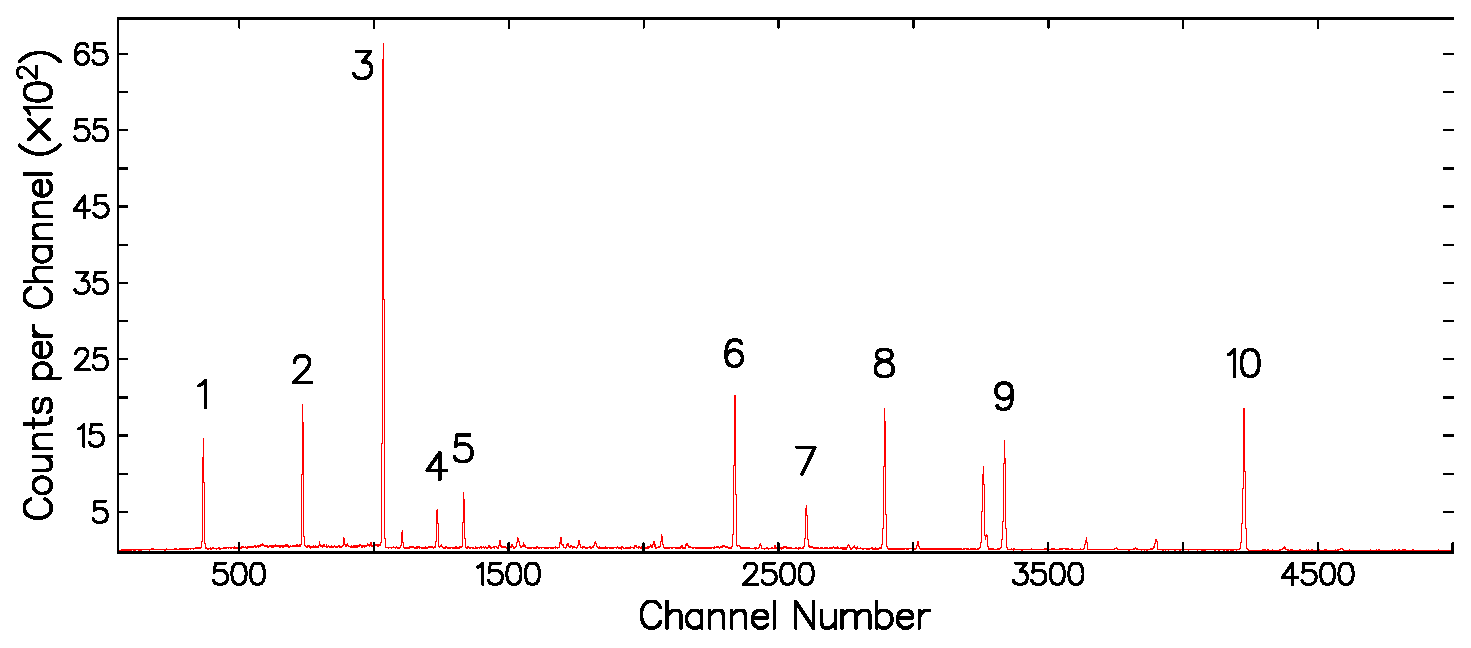
\includegraphics[height=0.25\textheight]{./img/c3/gs_cal_spec.eps}}
	\caption{$^{152}$Eu calibration spectrum from a typical Gammasphere detector.}
	\label{fig:chp3-gs-cal-spec}
	\setlength{\capwidth}{0.9\textwidth}
\end{figure}

\begin{figure}[h!]
	\centerline{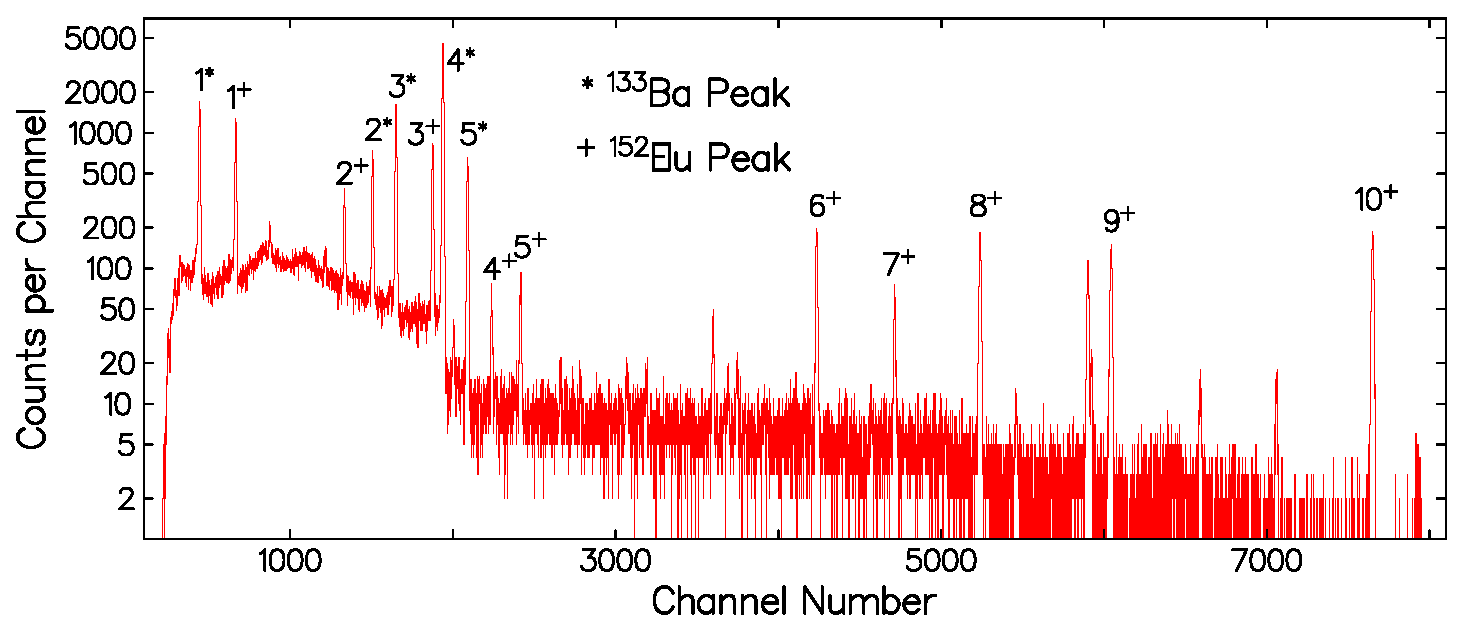
\includegraphics[height=0.25\textheight]{./img/c3/inga_crystal_en_cal.eps}}
	\caption{Typical $^{152}$Eu and $^{133}$Ba mixed source calibration spectrum from a single crystal of an INGA clover detector.}
	\label{fig:chp3-inga-cal-spec}
\end{figure}

For Gammasphere after extraction of the spectra, energy calibration of each detector was performed as follows. First, using the program \emph{gf3} from the Radware tool suite\cite{radware}, each of the $10$ peaks was fit with a Gaussian peak shape plus linear background whose formula is:
\begin{equation}
\label{eqn:chp3-pk_fit} 
Fit(x) = h e^{-\frac{(x-\mu{})^2}{2\sigma{}^2}} + a + b (x-\overline{x})
\end{equation}
 Where $x$ is the channel number, $h$ is the peak height, $\mu{}$ is the peak centroid, $2\sqrt{2ln(2)}\sigma{}$ is the FWHM of the peak, $a$ is the constant term of the background, $b$ is the linear term of the background, and $\overline{x}$ is the center of the region to be fitted. From these shapes the peak area ($\sqrt{2\pi{}}\sigma{}h$) and centroid were extracted. For energy calibration the centroids were combined with the corresponding energies and fitted with polynomials (as in eqn \ref{eqn:chp3-en_cal}) from $2^{nd}$ to $5^{th}$ order.

\begin{equation}
\label{eqn:chp3-en_cal} 
E = a_0 + a_1x + a_2x^2 + a_3x^3 + a_4x^4 + a_5x^5
\end{equation}

The reduced $\chi{}^2$ of the fitted polynomials ($\chi^2/d.o.f.$) were compared and the polynomial with the lowest reduced $\chi{}^2$ was selected to be the energy calibration for that detector. A listing of the energy calibration parameters used for Gammasphere is found in Table \ref{tbl:app1-gs-en-cal}.

For INGA, following the extraction of single crystal spectra, energy calibration was performed by using \emph{gf3} to fit each of the peaks of interest and extract the positions of each peak. After gathering the peak positions and combining them with their respective energies a $2^{nd}$ order polynomial was fit. No higher order polynomials were used due to both the enhanced linearity of a digital data acquisition system and limitations in the code used for further analysis. A listing of the energy calibration parameters used for INGA can be found in table \ref{tbl:app2-inga-en-cal}.

For Gammasphere the peak areas were divided by the corresponding relative intensities in Table \ref{tbl:152Eu-peaks} to give the relative efficiency of each peak, following energy calibration. Then, using the program \emph{effit} from the Radware suite, the energies and relative efficiencies of each peak were then fitted with:
\begin{equation}
\label{eqn:chp3-eff_cal} 
ln(\epsilon) = [(A+Bx+Cx^2)^{-G} + (D+Ey+Fy^2)^{-G}]^{-1/G}
\end{equation}
Here $A$, $B$, $C$ are parameters that control the low energy part of the efficiency, though $C$ is usually set to $0.0$. $D$, $E$, $F$ are the parameters that control the high energy component of the efficiency. $G$ is the parameter that controls the ``sharpness'' of the intermediate energy turnover region where they play equal roles. The parameters $x$ and $y$ are related to the \gr{} energy as follows:
\begin{align*}
\label{eqn:chp3-eff_x_and_y}
x=ln(\frac{E_{\gamma{}}}{100~keV}) && y=ln(\frac{E_{\gamma{}}}{1000~keV})
\end{align*}
A plot of extracted relative efficiencies and the fit to them for a Gammasphere detector can be found in Fig. \ref{fig:chp3-gs-eff-plot}. A listing of the relative efficiency calibration parameters used for Gammasphere is found in table \ref{tbl:app1-gs-en-cal}.

\begin{figure}[h!]
	\centerline{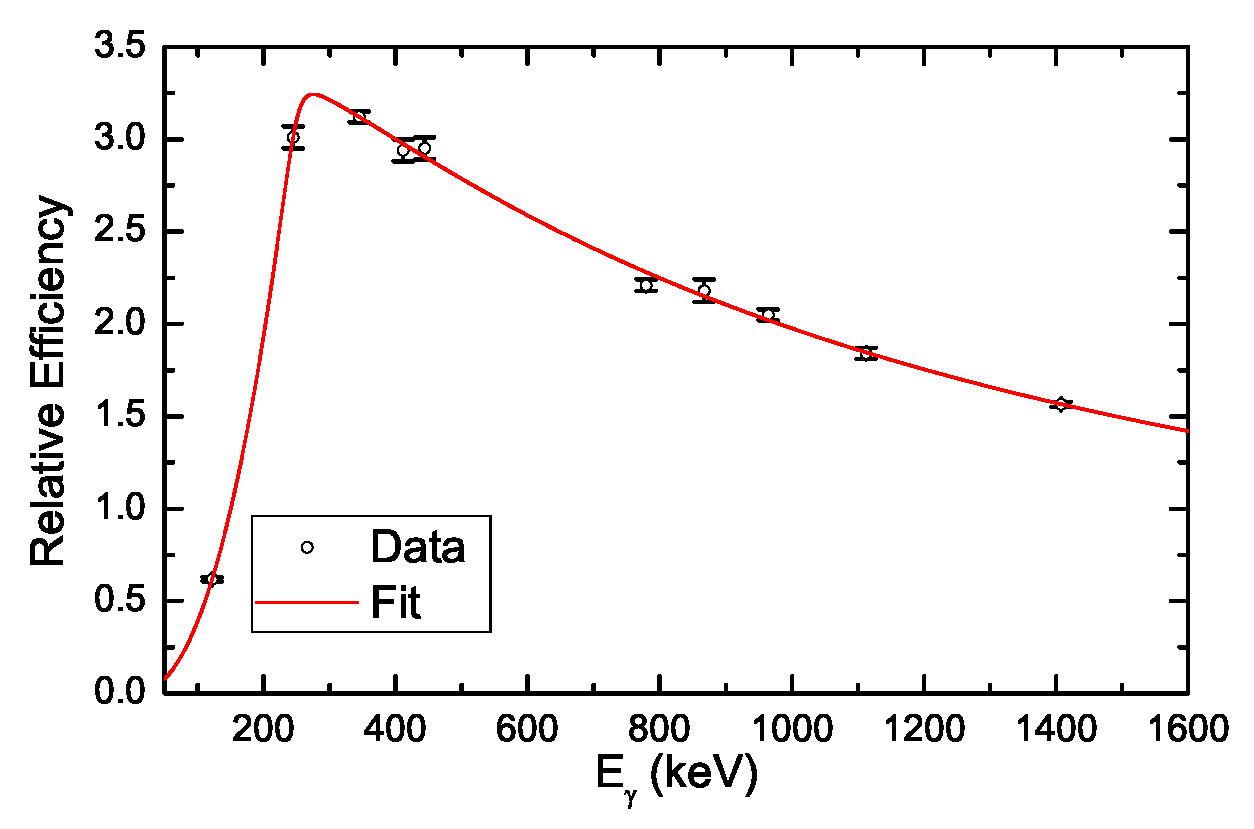
\includegraphics[width=0.9\textwidth]{./img/c3/gs_eff_plot.eps}}
	\caption{$^{152}$Eu extracted relative efficiencies and fit.}
	\label{fig:chp3-gs-eff-plot}
\end{figure}

As it was unnecessary for the asymmetry analysis performed on the INGA data a relative efficiency calibration was not performed. If it had been necessary, the ratio of the $^{133}$Ba and $^{152}$Eu source activities would have been needed or it would be necessary to include that ratio as an eighth parameter of the fit. This would allow normalization of the relative efficiencies of the peaks from the two sources to the same scale.

\subsection{Level Scheme Scheme Determination}
\label{ssec:exp-pr-data-proc-lvl-scheme}
The analysis of the Gammasphere thin target data involved extending known portions of the level scheme using the Radware software package\cite{radware}. Radware uses symmetrized multi-dimensional histograms to store high fold events. In these multidimensional arrays each axis corresponds to a \gr{} energy and each bin in the array corresponds to a event with that particular combination of \gr{} energies seen within a $1\mu{}s$ window. The histograms are symmetrized by sorting the \gr{} energies of each event such that $E_1\leq{}...\leq{}E_d$. In doing this number of bins in the histogram can be reduced from $n^d$ (where $n$ is the number of bins per axis and $d$ is the number of axes) to:
\begin{equation}
\label{eqn:chp3-hist-size}
Size=\frac{1}{d!}\prod\limits_{i=1}^{d}(n+i)
\end{equation}
While this still scales with $n^d$ it reduces somewhat the large storage requirements. Events that are of lower dimensionality than the histogram are ignored and events that are of higher fold than the histogram, $f$, are ``unfolded'' into $f \choose d$ unique events.

Reconstruction of a nucleus' level scheme involves gating on one or more transitions and examining the resultant spectra which will show what transitions are in coincidence with the gates. A gate on a symmetrized histogram is a projection of the histogram along one of its axes with restrictions on the summation of the other axes. As an example, equation \ref{eqn:chp3-matrix-proj}, shows a gateless projection of a matrix ($2-d$ histogram). Equation \ref{eqn:chp3-matrix-single-gate} shows a single gate on a matrix.
\begin{equation}
\label{eqn:chp3-matrix-proj}
S_i = \sum\limits_{j=0}^{n-1}M_{ij}
\end{equation}
\begin{equation}
\label{eqn:chp3-matrix-single-gate}
S^{g_1}_i = \sum\limits_{j=g_{lo}}^{g_{hi}}M_{ij}
\end{equation}
Here $S_i$ is the counts bin $i$ in the resultant spectrum, $S^{g_1}_i$ is the counts of bin $i$ in the gated spectrum, $M_{ij}$ is the counts at bin $i,j$ in the matrix, $g_{lo}$ and $g_{hi}$ are the bounds of the gate, and $n$ is the number of bins per axis of the matrix. Expressions for higher order gates and higher dimensional histograms follow logically from these expressions.

The peaks in the spectrum yielded by gating on one or more \gr{}s correspond to the \gr{}s that are in coincidence with the gated \gr{}s. If two transitions are in coincidence, they must all be part of the same cascade through the level scheme. Therefore, at \emph{least} individually, each of the peaks in the gated spectrum will be part of the same cascades as the \gr{} that were chosen for the gate. By varying which \gr{} are gated upon and observing the intensity of the gated transitions it is possible to determine the placement of essentially all the \gr{} transitions in the level scheme.

\subsection{Background Subtraction}
\label{ssec:exp-pr-data-proc-bg-sub}
A spectrum can be thought of as having two components, the background part and the peak part. Any given segment of this background is made from \gr{}s that were in random/``accidental'' coincidence and \gr{} that were in true coincidence and only deposited part of their energy in the detector. When a gate is placed on an energy range, the gate is on both peak and background components. In addition to this the \gr{}s that are in coincidence with a gate are likewise composed of background and peak themselves. The removal of these backgrounds is vital in the analysis of \gr{} coincidence data.

\subsubsection{Symmetric Gates}
\label{sssec:exp-pr-data-proc-bg-sub-sym}
For symmetric gates where all the axes can be taken to be equivalent, the background developed by Radford in Ref. \cite{symBGSub} is used. For a cube ($3-d$ histogram) this background is:
\begin{equation}
\label{eqn:chp3-cube-bg}
B_{ijk}=\frac{1}{T}\left(M_{ij}b_{k} + M_{ik}b_{j} + M_{jk}b_{i}\right) + \frac{1}{T^{2}}\left(b_{i}b_{j}b_{k} - P_{i}b_{j}b_{k} - b_{i}P_{j}b_{k} - b_{i}b_{j}P_{k}\right)
\end{equation} 
Here $M_{ij}$ is two dimensional projection of the cube, $P_{i}$ is the projection of the cube, $b_{i}$ is the smooth background component of the cube's projection, and T is the total counts in the cube.
\begin{align}
\label{eqn:chp3-cube-bg-defs}
M_{ij} &= \sum\limits_{k}^{}C_{ijk} \\
P_i &= p_i + b_i = \sum\limits_{jk}^{}C_{ijk}\\
T &= \sum\limits_{ijk}^{}C_{ijk}
\end{align}

Similar expressions are derived for gates on matrices and hypercubes ($4-d$ histograms) in Ref \cite{symBGSub}. The extraction of the smooth background component $b_{i}$ from the total projection $P_{i}$ can be seen in  Fig. \ref{fig:chp3-smooth-bg}. An example of the background from this procedure and the results of the subtraction can be seen in Fig. \ref{fig:chp3-sym-bg-sub}. 
\begin{figure}[h!]
	\centerline{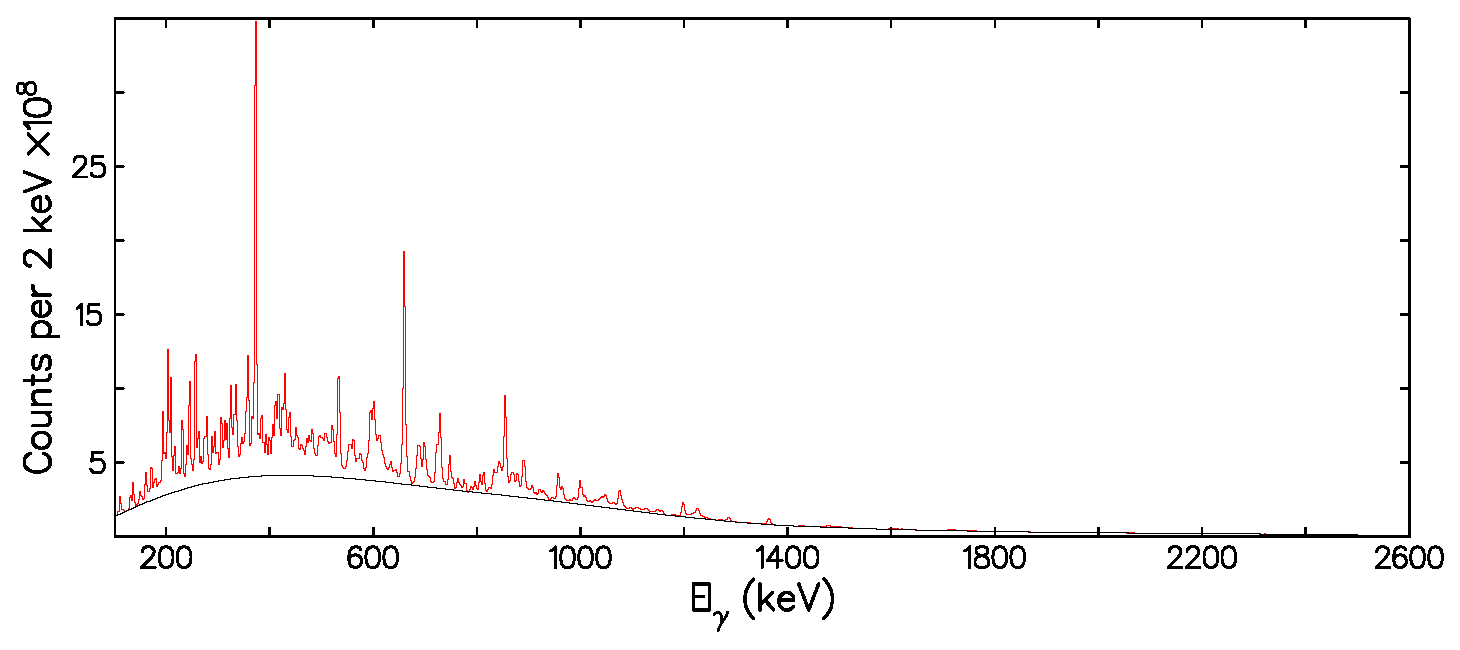
\includegraphics[width=0.6\textwidth]{./img/c3/smth_bg.eps}}
	\caption{Total projection spectrum and its smooth background drawn below it.}
	\label{fig:chp3-smooth-bg}
\end{figure}

\begin{figure}[h!]
	\centerline{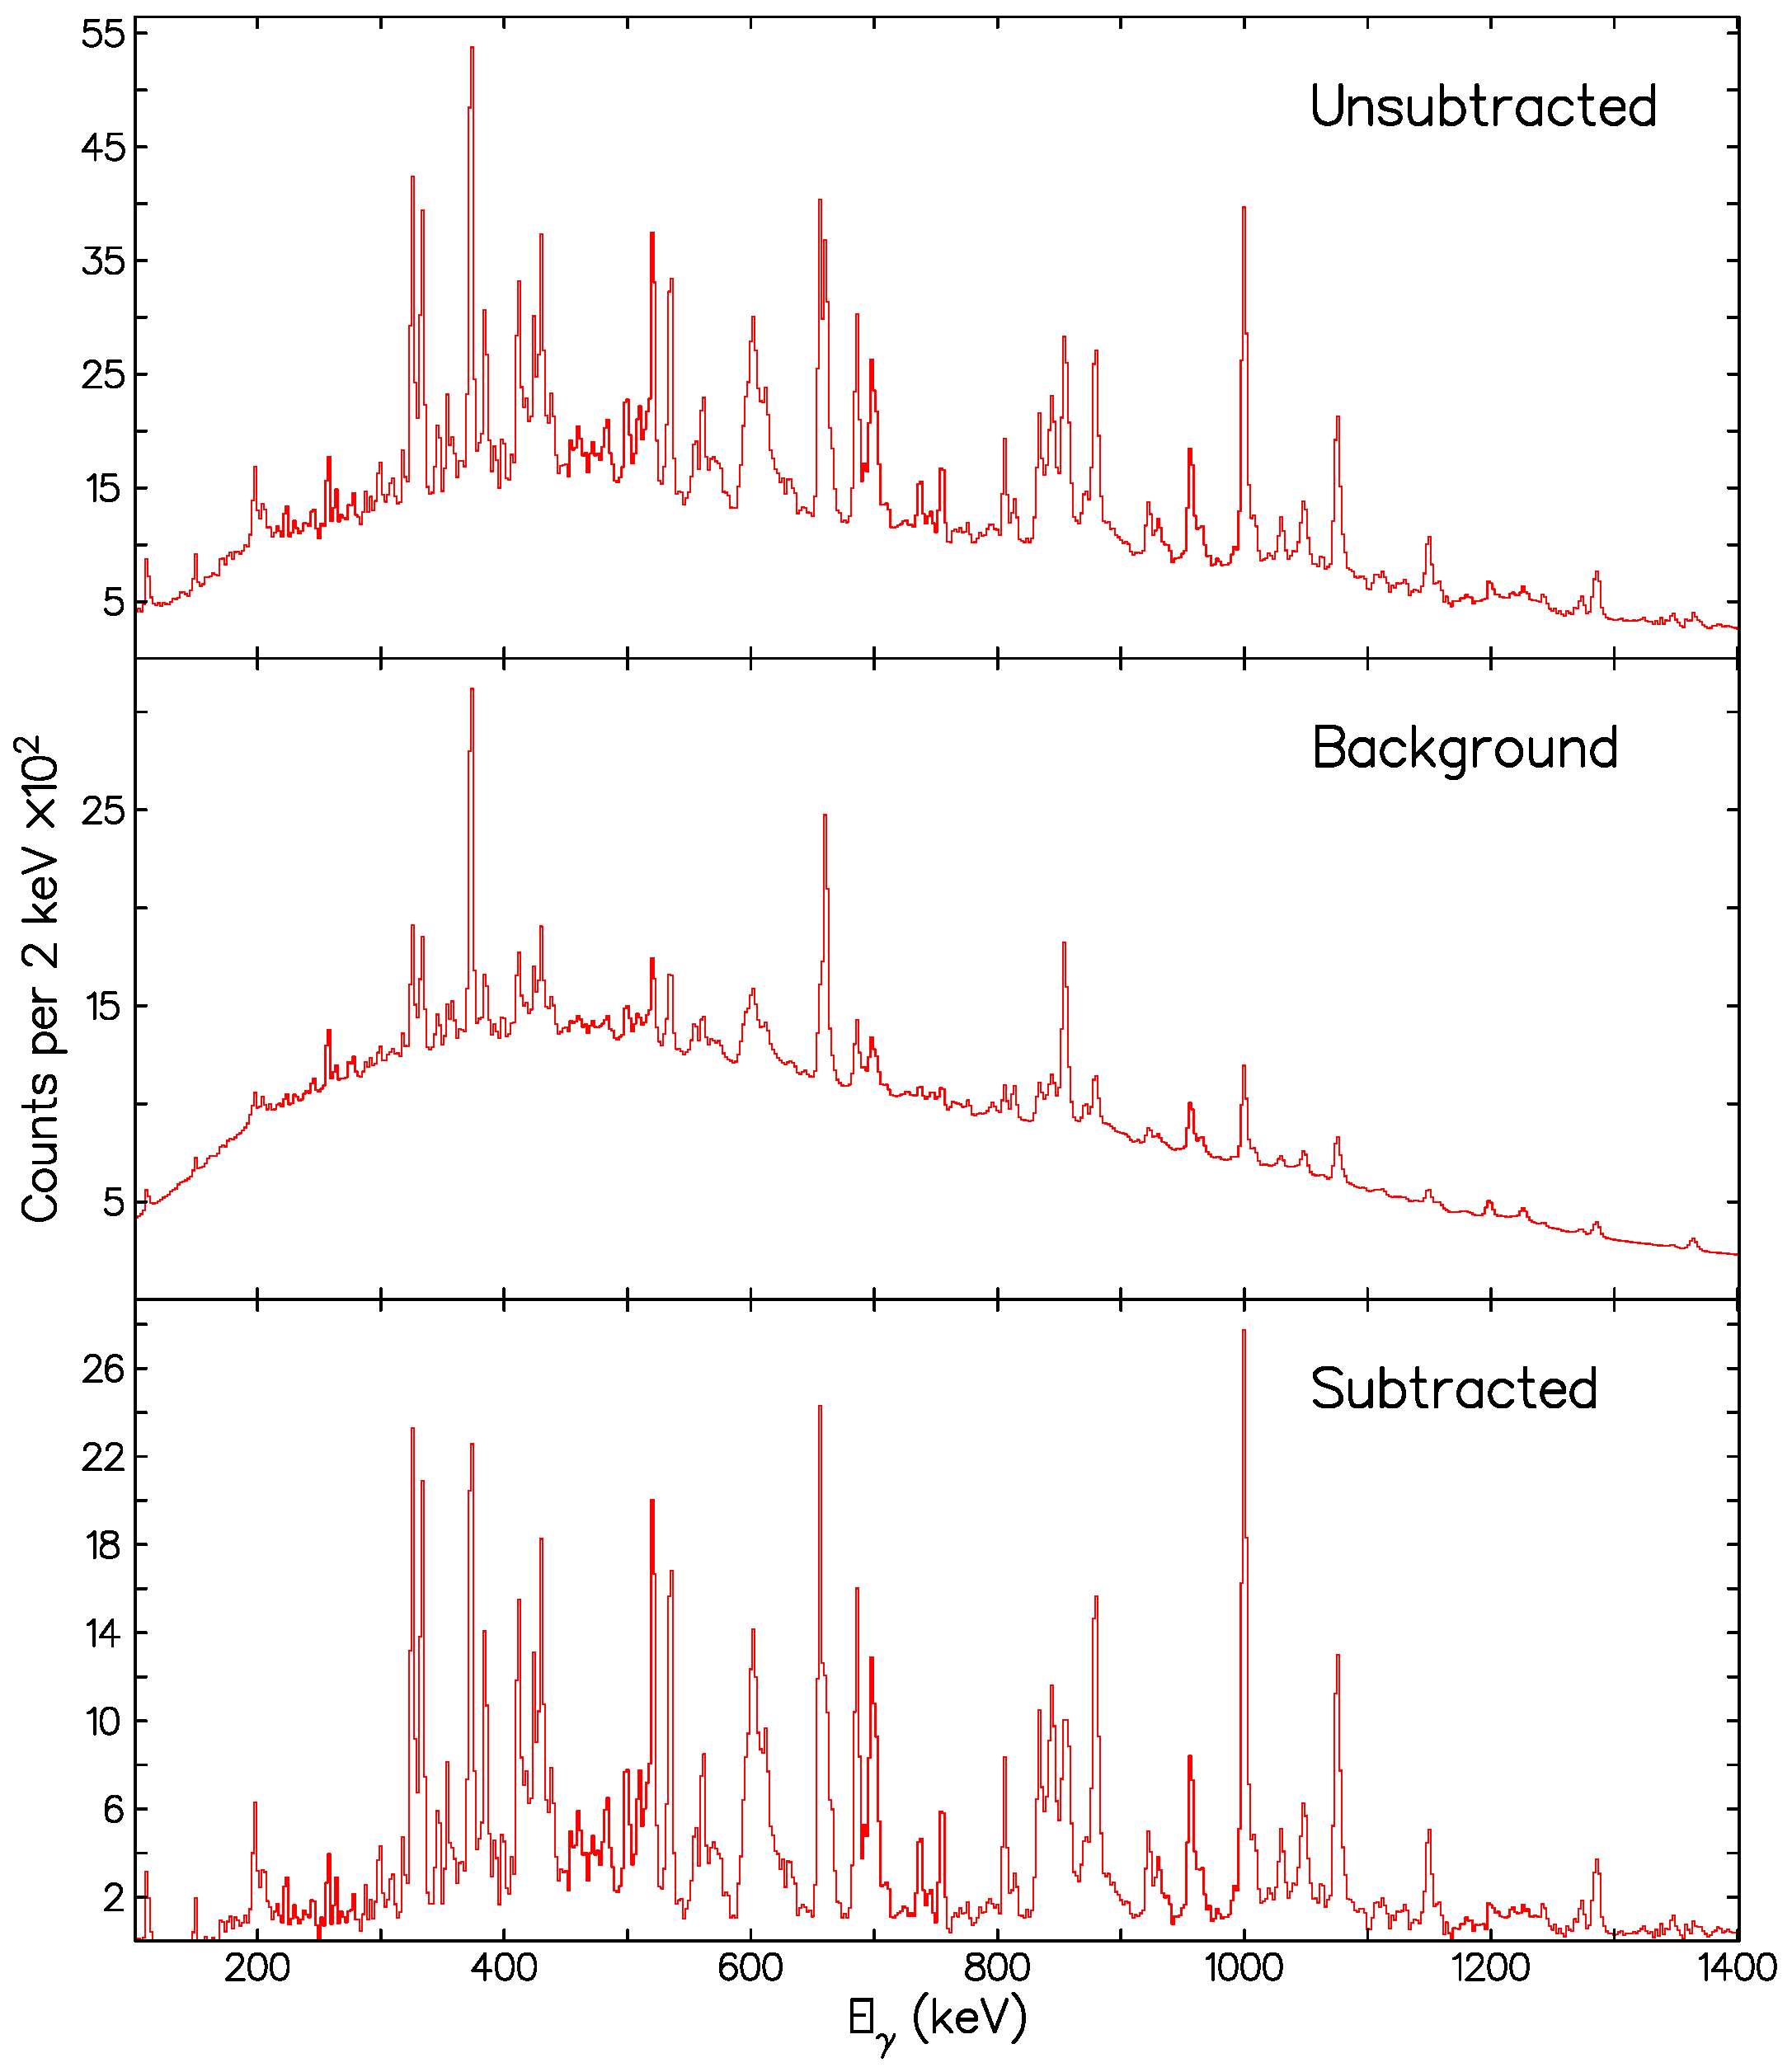
\includegraphics[width=0.6\textwidth]{./img/c3/bg_sub_ex.eps}}
	\caption{Spectra of a symmetric triple gate on a hypercube showing the components of the gates spectrum. Top: The unsubtracted gated spectrum. Middle: The background spectrum for the gate. Bottom: The final background subtracted spectrum.}
	\label{fig:chp3-sym-bg-sub}
\end{figure}

\subsubsection{Asymmetric Gates}
\label{sssec:exp-pr-data-proc-bg-sub-asym}
Some types of data analysis, such as those examined in Section \ref{sec:exp-pr-data-ang}, require asymmetric gates where the $\uvec{x}$-axis of the spectrum produced is not the same as the axes that were gated on/summed across. For example the projection axis is gammas seen in a specific ring of the array while the gate is placed on all the rings of the array. In such cases the background subtraction method developed by Starosta et al. in Ref \cite{asymBGSub} is necessary. If one considers a double gate on $\gamma{}_1$ and $\gamma{}_2$, then events in that double gate will fall into four categories:
\begin{enumerate}
\item[$1$:pp] Peak-Peak: Both $\gamma{}_1$ and $\gamma{}_2$ are correctly identified.
\item[$2$:pb] Peak-Background: $\gamma{}_1$ is correctly identified and $\gamma{}_2$ comes from background.
\item[$3$:bp] Background-Peak: $\gamma{}_1$ is from background and $\gamma{}_2$ is correctly identified.
\item[$4$:bb] Background-Background: Both $\gamma{}_1$ and $\gamma{}_2$ are from background.
\end{enumerate}
Similar combinations apply to higher order and lower order gates. The spectrum to examined should be made up solely of events from the first category. To subtract events that fall into categories $2$, $3$, and $4$ we first realize:
\begin{align}
S_{pp}(j) &= S_{tt}(j) - B_{\gamma{}\gamma{}}(j)\label{eqn:chp3-asym-pp}\\
B_{\gamma{}\gamma{}}(j) &= N_{bp}S_{bp}(j) + N_{pb}S_{pb}(j) + N_{bb}S_{bb}(j)\label{eqn:chp3-asym-gg}\\
N &= N_{pp} + N_{pb} + N_{bp} + N_{bb} \label{eqn:chp3-asym-N}
\end{align}
$S_{pp}$ is the spectrum corresponding to events that are in the first category, $S_{tt}$ is the spectrum of all events that satisfy the gate, $N_{x}$ is the number of events in category $x\in{}\{pp,pb,bp,bb\}$, and $S_{x}$ is the spectrum of events that falls into category $x$, normalized to have a total of $1$ count.

With the assumption that the background is uncorrelated it follows that for category $bb$ the corresponding spectrum will be proportional to the total projection spectrum. This assumption also gives that the spectra for categories $pb$ and $bp$ will be proportional to the background subtracted spectra of a single gate on those peaks. From this we have the following relations:
\begin{align}
S_{bb}(j) &=\frac{1}{T}P(j) & T &= \sum\limits_{j}^{}P(j) \label{eqn:chp3-asym-bb}\\
S_{pb} &= \frac{1}{N^{g_1}_{BgSub}}S^{g_1}_{BgSub}(j)  & N^{g_1}_{BgSub} &= \sum\limits_{j}^{}S^{g_1}_{BgSub}(j) \label{eqn:chp3-asym-bp}\\
S_{bp} &= \frac{1}{N^{g_2}_{BgSub}}S^{g_2}_{BgSub}(j)  & N^{g_2}_{BgSub} &= \sum\limits_{j}^{}S^{g_2}_{BgSub}(j) \label{eqn:chp3-asym-pb}\\
S^{g_i}_{BgSub}(j) &= S^{g_i}(j) - b_i \frac{N_{g_i}}{T}P(j) & N_{g_i} &=  \sum\limits_{j}^{}S^{g_i}(j)  \label{eqn:chp3-asym-sg-bgsub}
\end{align}
Where $S^{g_i}$ are the unsubtracted, unnormalized spectra resulting from a single gate on a single transition, $P(j)$ is the total projection spectrum of all gamma multiplicities the gate is applied to, and $b_i$ is the background to total ratios of peak $i$ of the peaks that were gated on, extracted via the standard methods, \emph{eg} Fig. \ref{fig:chp3-asym-bg-ratio}. It is also worth noting that $N^{g_i}_{BgSub} = N_{g_i}(1 - b_i)$, combining this with equations \ref{eqn:chp3-asym-pp} through \ref{eqn:chp3-asym-sg-bgsub} yields the for $B_{\gamma{}\gamma{}}(j)$ given in \ref{eqn:chp3-asym-bg-dg-exp}.

\begin{figure}[h!]
	\centerline{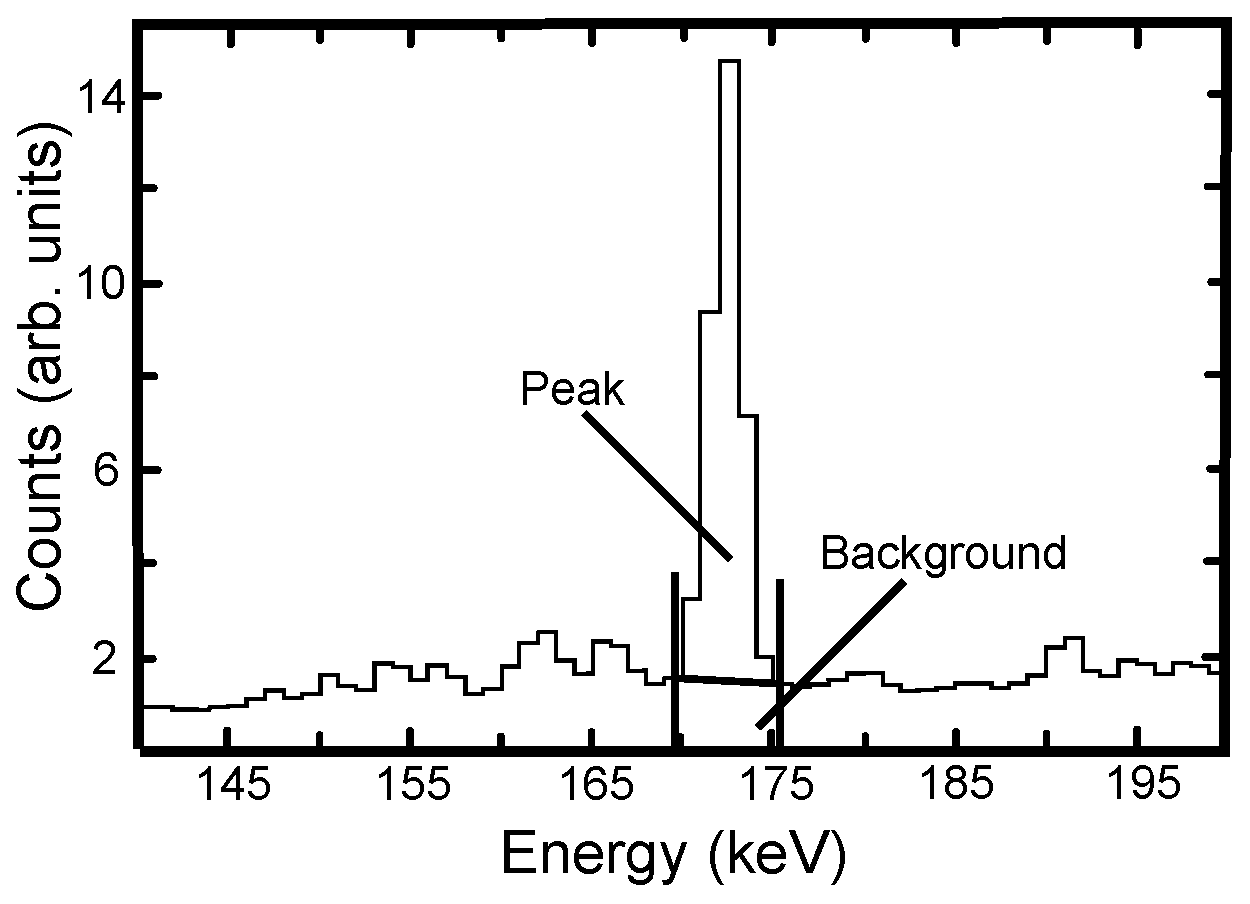
\includegraphics[width=0.6\textwidth]{./img/c3/peak_to_bg_asym_bg.eps}}
	\caption{Extraction of the peak and background, where $p + b = 1$. Adapted from Ref. \cite{asymBGSub}.}
	\label{fig:chp3-asym-bg-ratio}
\end{figure}

\begin{equation}
\label{eqn:chp3-asym-bg-dg-exp}
B_{\gamma{}\gamma{}}(j)=N\left(\frac{b^{g_1}_2}{N^{g_1}}S^{g_1}(j) + \frac{b^{g_2}_1}{N^{g_2}}S^{g_2}(j) - \frac{b_1b^{g_1}_2+b_2b^{g_2}_1}{2T}P(j) \right)
\end{equation}
Where $b^{g_k}_i$ is the background to total ratio of peak $i$ in $S^{g_k}(j)$, extracted similarly to the $b_i$ of Equation \ref{eqn:chp3-asym-sg-bgsub}. This expression removes spurious correlations which arise from the background components of the gating transition(s). However, there is a further smooth background that results from the incomplete suppression of escapes. This smooth background can be accounted for in one of two ways. The first is to remove it via the prescription shown in Ref. \cite{asymBGSub}, which uses a scaled smooth background of the total projection, like that in Fig. \ref{fig:chp3-smooth-bg}. The second method is to account for it locally with a background term in during peak fitting. In the case of this work, the latter method was chosen for simplicity.

\section{Directional Correlation of Gamma-rays from Oriented Nuclei (DCO)}
\label{sec:exp-pr-data-ang}
Angular distribution measurements, angular correlation measurements, and polarization measurements all rely on the nucleus which emits the radiation, being oriented in some fashion. There are three broad categories of methods for establishing the orientation of the nucleus. The first category involves using a beam to impose an orientation via nuclear reaction (such as fusion-evaporation) or coulomb excitation. In the second category a sample of radioactive atoms that have non-zero spin are cryogenically cooled and an external magnetic field is applied. The spins align in this field to the extent determined by their temperature and the field strength. The final category involves, not forcing the nucleus into some orientation, but observing its orientation by taking the direction of a radiation preceding the \gr{} of interest to be the $\uvec{z}$-axis. A diagrammatic scheme for the emission of two successive radiations $X_1$ and $X_2$ is found in Fig. \ref{fig:chp3-DCO-diagram-lvl-scheme}.

\begin{figure}[h!]
	\centerline{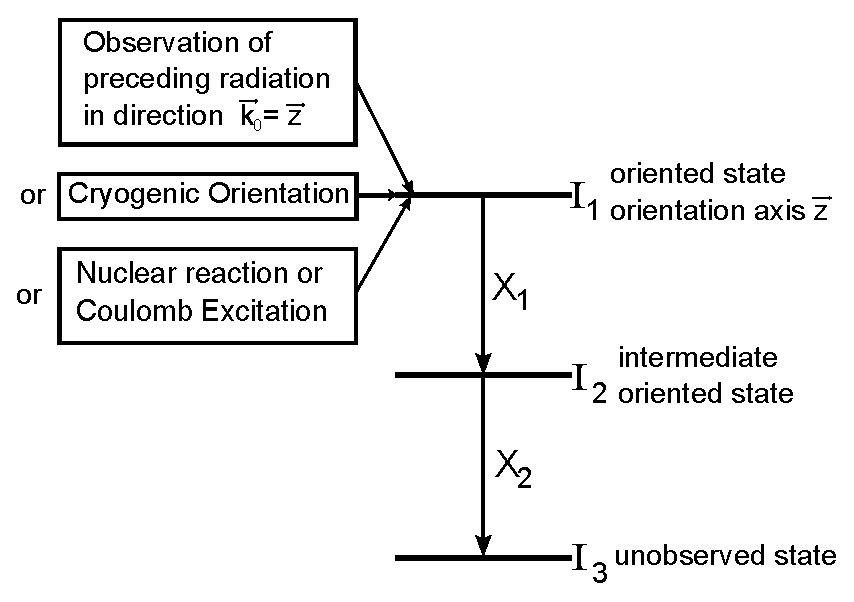
\includegraphics[height=0.35\textheight]{./img/c3/dco_lvl_scheme.eps}}
	\caption{Emission of two successive radiations $X_1$ and $X_2$ from an oriented nuclear state, $I_1$.}
	\label{fig:chp3-DCO-diagram-lvl-scheme}
\end{figure}

The full correlation function describing the situation in Fig. \ref{fig:chp3-DCO-diagram-lvl-scheme} can be written as follows\cite{dcoKrane,emInteraction}:
\begin{equation}
\label{eqn:chp3-full-dco}
W\left(\theta{}_1,\theta{}_2,\phi{}\right) = \sum\limits_{\lambda{}_1,\lambda{},\lambda{}_2}^{} B_{\lambda{}_1}\left(I_1\right) A_{\lambda{}}^{\lambda{}_2\lambda{}_1}\left(X_1\right) A_{\lambda{}_2}\left(X_2\right) H_{\lambda{}_1\lambda{}\lambda{}_2}\left(\theta{}_1,\theta{}_2,\phi{}\right)
\end{equation}
Here $\lambda{}_1$ and $\lambda{}_2$ are the ranks of the statistical tensors that describe the orientation of states $I_1$ and $I_2$, $\lambda{}$ is the tensor rank of the radiation field, $B_{\lambda{}_1}\left(I_1\right)$ is the orientation coefficient, $A_{\lambda{}}^{\lambda{}_2\lambda{}_1}\left(X_1\right)$ is the generalized directional distribution coefficient, $A_{\lambda{}_2}\left(X_2\right)$ is the directional distribution coefficient, and $H_{\lambda{}_1\lambda{}\lambda{}_2}\left(\theta{}_1,\theta{}_2,\phi{}\right)$ is the angular function defined in Eqn. \ref{eqn:chp3-angular-function}. The angles referenced in Eqns. \ref{eqn:chp3-full-dco} and \ref{eqn:chp3-angular-function} are defined in Fig. \ref{fig:chp3-DCO-Angles}. Additionally, $X_i$ corresponds to a listing of the pertinent information about the $i^{th}$ radiation, namely $X_i = \left(\delta{}_i,L_i,L'_i,I_{i+1},I_i\right)$. Here $L_i$ is the low-order multipolarity of radiation $i$, $L'_i$ is the high-order multipolarity of radiation $i$, $\delta{}_i$ is the mixing ratio between the two multipolarities, $I_i$ is the initial state for the radiation, and $I_{i+1}$ is the final state for the radiation. The mixing ratio $\delta{}$ is defined as a ratio of matrix elements as in Eqn. \ref{eqn:chp3-mixing-ratio-matrix} or as the square root of a ratio of intensities as in Eqn. \ref{eqn:chp3-mixing-ratio-inten}. While it is possible to define formulae for $B_{\lambda{}_1}\left(I_1\right)$, $A_{\lambda{}}^{\lambda{}_2\lambda{}_1}\left(X_1\right)$, and $A_{\lambda{}_2}\left(X_2\right)$ to accommodate three multipolarity components, a situation where the highest order component is strong enough to require accounting for is extremely unlikely and so henceforth only equations for two components will be given.
\begin{align}
\delta{} &= \frac{<I_2||\boldmath{j_NA^{\pi{}'}_{L'}}||I_1>}{<I_2||\boldmath{j_NA^{\pi{}}_{L}}||I_1>} \label{eqn:chp3-mixing-ratio-matrix}\\
\delta{} &= \sqrt{\frac{I_{\gamma{}}(L')}{I_{\gamma{}}(L)}} \label{eqn:chp3-mixing-ratio-inten}
\end{align}

\begin{equation}
\label{eqn:chp3-angular-function}
H_{\lambda{}_1\lambda{}\lambda{}_2}\left(\theta{}_1,\theta{}_2,\phi{}\right) = \sum\limits_{q=-\lambda{}'}^{\lambda{}'}\frac{4 \pi{}}{2\lambda{}_2 +1} <\lambda{}_1 0 \lambda{} q | \lambda{}_2 q> Y_{\lambda{}q}\left(\theta{}_1,0\right) Y^{*}_{\lambda{}q}\left(\theta{}_2,\phi{}\right)
\end{equation}

\begin{figure}[h!]
	\centerline{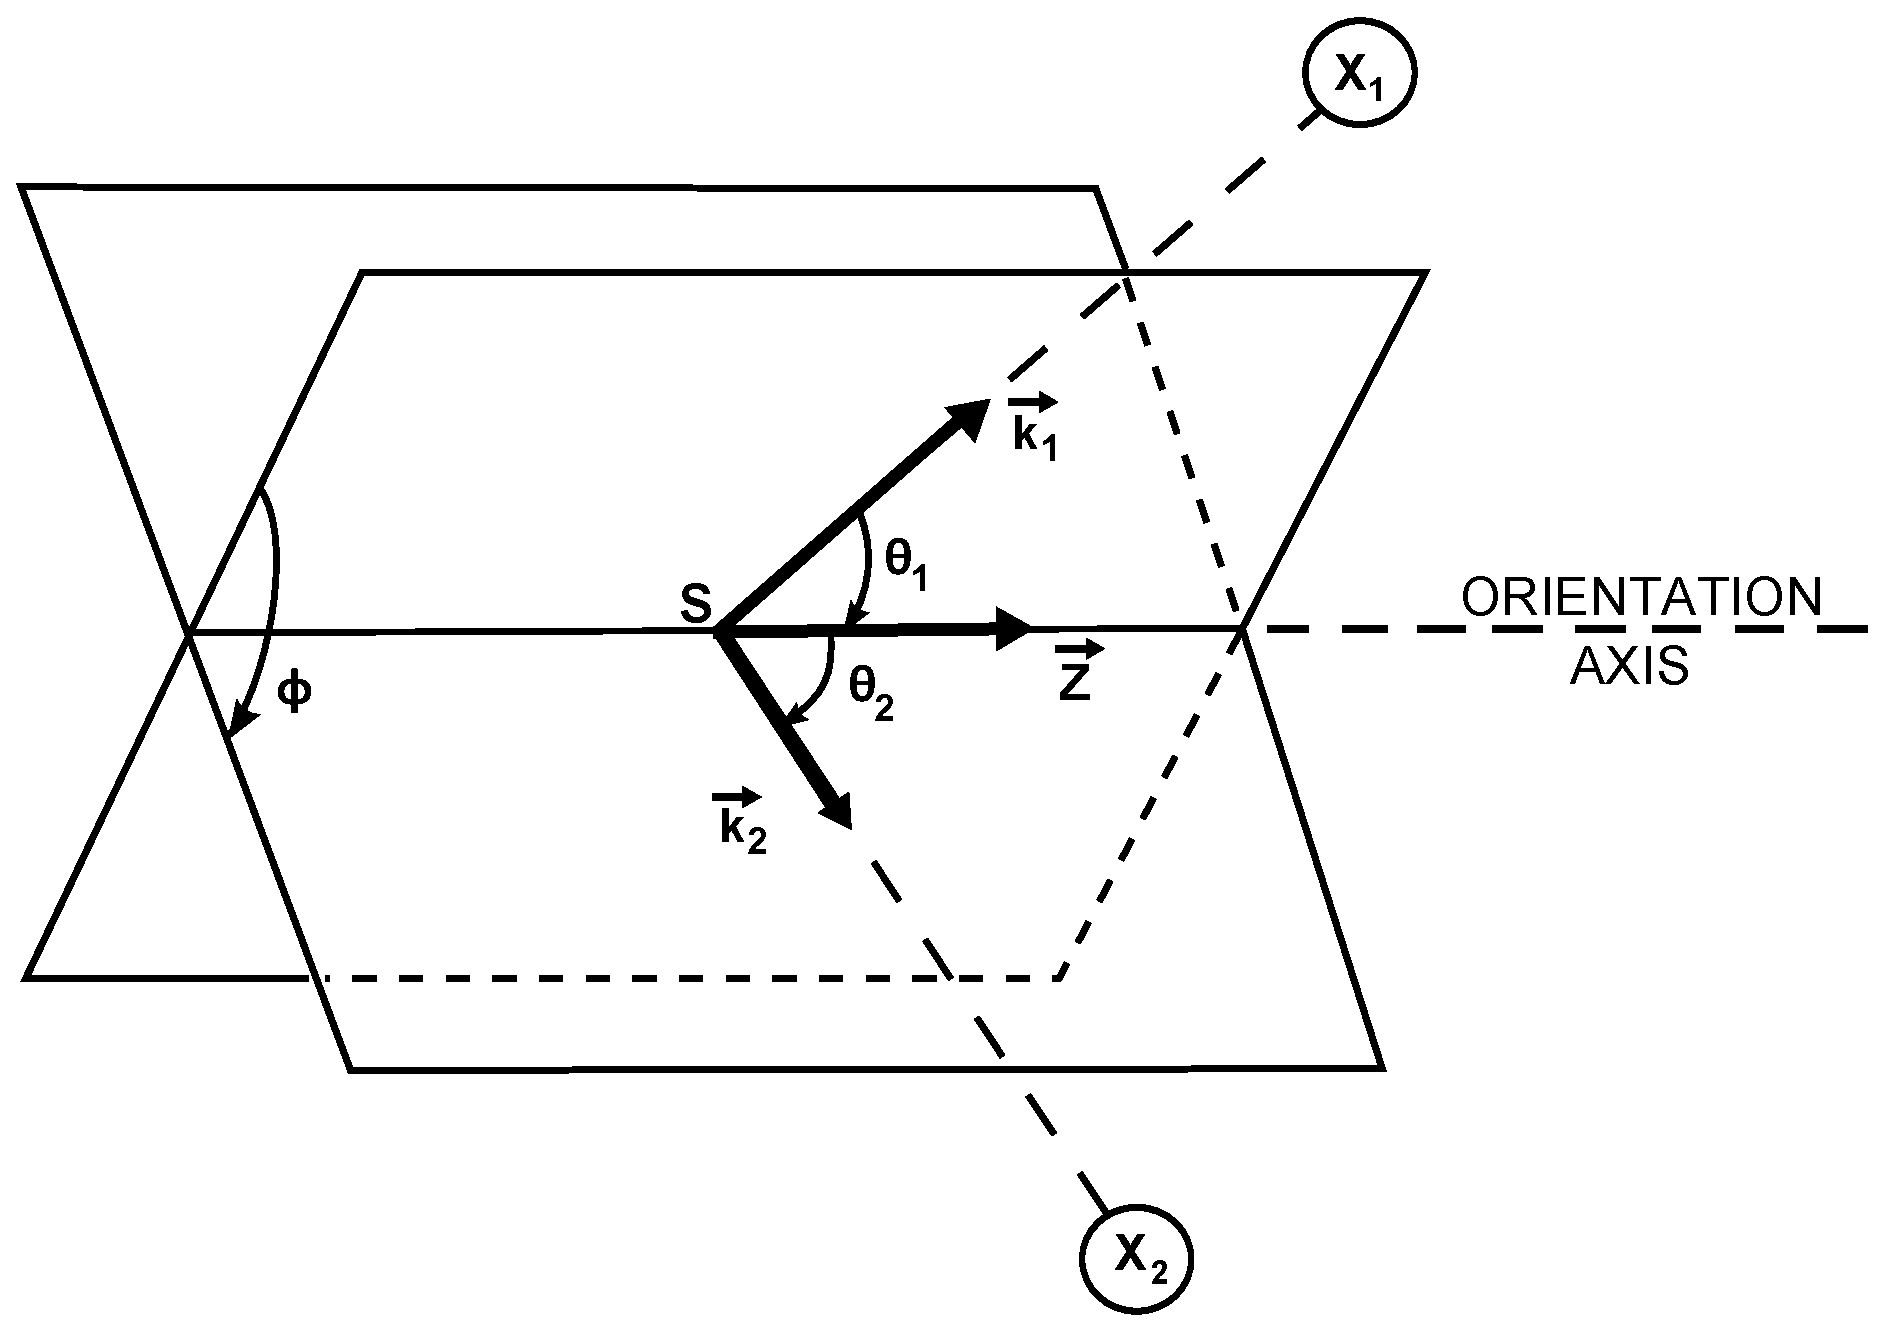
\includegraphics[height=0.35\textheight]{./img/c3/dco_setup.eps}}
	\caption{Diagram of the angles in a directional correlation of two successive radiations X$_{1}$ and X$_{2}$ emitted from an axial symmetric oriented source S.}
	\label{fig:chp3-DCO-Angles}
\end{figure}

The orientation parameters $B_{\lambda{}_1}\left(I_1\right)$ take several different forms depending on the method used to orient the nucleus. For methods which result in an axially symmetric distribution where the nucleus has probability $P(m)$ to be in a given magnetic substate $m$, Eqn. \ref{eqn:chp3-orient-fus-evap} is used. For determining the orientation of the nucleus by observing a preceding \gr{} $X_0$, Eqn. \ref{eqn:chp3-orient-preceding} is used.

\begin{align}
B_{\lambda{}}\left(I_1\right) &= \sqrt{2I_1+1}\sum\limits_{m}^{}(-1)^{I_1+m} \times{}<I_1 -m I_1 m | \lambda{} 0> P(m) \label{eqn:chp3-orient-fus-evap}\\
B_{\lambda{}}\left(I_1;X_0\right) &= \frac{F_{\lambda{}}(L_0 L_0 I_0 I_1) + 2 \delta{} F_{\lambda{}}(L_0 L'_0 I_0 I_1) + \delta{}^2 F_{\lambda{}}(L'_0 L'_0 I_0 I_1)}{1+\delta{}^2} \label{eqn:chp3-orient-preceding}
\end{align}
In the case of a fusion-evaporation reaction, the probability function $P(m)$ is assumed to be of the form of a Gaussian distribution\cite{angDist} which yields:
\begin{equation}
\label{eqn:chp3-fe-prob-func}
P(m,J,\sigma) = \frac{e^{-m^2/(2\sigma{}^2)}}{\sum\limits_{m'=-J}^{J}e^{-m^2/(2\sigma{}^2)}}
\end{equation}
Here $\sigma$ is the width of the distribution (thus $\sigma{}=0$ corresponds to perfect alignment of the ensemble of nuclei), $J$ is the spin of the initial state, and $m$ is the substate index. $\sigma$ is usually fit to be a function of the initial state's spin $J$ in the form $\sigma{}=C*J$. The parameter $C$ is usually in the range of $0.2$ to $0.4$ for typical fusion-evaporation reactions.

The directional distribution coefficients, generalized and otherwise, are defined as:
\begin{align}
A_{\lambda{}}^{\lambda{}_2\lambda{}_1}\left(X_1\right) &= \frac{F_{\lambda{}}^{\lambda{}_2\lambda{}_1}(L_1 L_1 I_2 I_1) + 2 \delta{} F_{\lambda{}}^{\lambda{}_2\lambda{}_1}(L_1 L'_1 I_2 I_1) + \delta{}^2 F_{\lambda{}}^{\lambda{}_2\lambda{}_1}(L'_1 L'_1 I_2 I_1)}{1+\delta{}^2}\label{eqn:chp3-gen-ddc}\\
A_{\lambda{}_2}\left(X_2\right) &= \frac{F_{\lambda{}}(L_2 L_2 I_3 I_2) + 2 \delta{} F_{\lambda{}}(L_2 L'_2 I_3 I_2) + \delta{}^2 F_{\lambda{}}(L'_2 L'_2 I_3 I_2)}{1+\delta{}^2} \label{eqn:chp3-ddc}
\end{align}

Here, the $F_{\lambda{}}^{\lambda{}_2\lambda{}_1}$ is the generalized $F$-coefficients and $F_{\lambda{}}$ is the ordinary $F$-coefficients.

The $F$-coefficients are defined as:
\begin{align}
F_{\lambda{}}^{\lambda{}_2\lambda{}_1}(L L' I_2 I_1) &=[(2I_1+1)(2I_2+1)(2L+1)(2L'+1)(2\lambda{}+1)\nonumber \\ & \times{} (2\lambda{}_1+1)(2\lambda{}_2+1)]^{1/2} (-1)^{L'+\lambda{}+\lambda{}_2+1}\nonumber \\
& \times{} \left(\begin{array}{clcr}L & L' & \lambda{}\\ 1 & -1 & 0  \end{array}\right) \left\{\begin{array}{clcr}I_2 & L & I_1\\ I2 & L' & I_1\\ \lambda{}_2 & \lambda{} & \lambda{}_1 \end{array}\right\} \label{eqn:chp3-gen-fcoef}\\
F_{\lambda{}}(L L' I_2 I_1) &= F_{\lambda{}}^{0\lambda{}}(L L' I_2 I_1)\label{eqn:chp3-fcoef}
\end{align}
Here $(...)$ is the Wigner-3j symbol and $\{ ... \}$ is the Wigner-9j symbol.

\subsection{Angular Distributions}
\label{ssec:exp-pr-data-ang-dist}
Angular distributions are the observation of the intensity distribution of single transitions relative to an orientation axis which has been set via a reaction or cryogenic methods. This is equivalent to saying that radiation $X_2$ was not observed which forces $\lambda{}_2=0$. Happily, under this requirement equation \ref{eqn:chp3-full-dco} simplifies dramatically. The angular function $H_{\lambda{}_1\lambda{}\lambda{}_2}\left(\theta{}_1,\theta{}_2,\phi{}\right)$ reduces to:
\begin{equation}
\label{eqn:chp3-simple-ang-func}
H_{\lambda{}_1\lambda{}0}\left(\theta{}_1,\theta{}_2,\phi{}\right) = P_{\lambda{}}(Cos[\theta{}_1])\delta_{\lambda{}\lambda{}_1}
\end{equation}
Here $P_{\lambda{}}$ is the Legendre polynomial and $\delta_{\lambda{}\lambda{}_1}$ is the Kronecker delta function. Furthermore the directional coefficients reduce in complexity as well:
\begin{align}
A_{\lambda{}}^{0\lambda{}_1}\left(X_1\right) &= A_{\lambda{}_1}\left(X_1\right)\delta_{\lambda{}\lambda{}_1} \label{eqn:chp3-gen-ddc-red}\\
A_{0}\left(X_2\right) &= 1 \label{eqn:chp3-ddc-red}
\end{align}
Together this gives us the distribution function of \cite{angDist}, namely:
\begin{equation}
\label{eqn:chp3-ang-dist}
W(\theta{}) = \sum\limits_{\lambda even}^{} B_{\lambda{}}\left(I_1\right) A_{\lambda{}}\left(X_1\right) P_{\lambda{}}(Cos[\theta{}])
\end{equation}

With this the angular distribution of \gr{} relative to the beam axis is fitted with:
\begin{equation}
\label{eqn:chp3-ang-dist-fit}
W(\theta{}) = A_{0}(1 + A_{2} P_{2}(Cos[\theta{}]) + A_{4} P_{4}(Cos[\theta{}]) ...)
\end{equation}

Here $A_{0}$ represents the normalized intensity obtained from peak areas in the \gr{} spectra. By analogy to Eqn. \ref{eqn:chp3-ang-dist} the $A_{\lambda{}}$ of the fit will depend on the orientation coefficient (and thus the degree of alignment), the spins of the original and final states, and the mixing ratio and multipolarity of the \gr{}. Typical ranges of values for various transitions can be seen in Table \ref{tbl:chp3-ang-dis-fit-ranges}. For high efficiency multi-detector arrays such as Gammsphere it is difficult, if not impossible, to extract \gr{} intensities from singles spectra due to the high complexity of total measured spectra. However, Ref \cite{angDistGates} shows that it is possible to place a quasi-isotropic gate on a transition preserves the angular distributions information of transitions higher in the cascade. Therefore it is possible to study angular distributions of \gr{}s that are weak or contaminated in the singles spectra by gating on a \gr{} below them to increase the signal to noise ratio or to remove the contamination.

\begin{table}[t]
\setlength{\abovecaptionskip}{-2pt}   % 0.5cm as an example
\setlength{\belowcaptionskip}{0.5pt}
\caption[\uppercase{Typical values of angular distribution coefficients $A_2$, $A_4$ for gamma-rays with Dipole (D), Quadrupole (Q), or mixed Dipole-Quadrupole Multipolarity, $l$.}]{\uppercase{Typical values of angular distribution coefficients $A_2$, $A_4$ for gamma-rays with Dipole (D), Quadrupole (Q), or mixed Dipole-Quadrupole Multipolarity, $l$.  Taken from} Ref.~\cite{angDistAVals}} \label{tbl:chp3-ang-dis-fit-ranges}
\centering
\begin{tabular}{c@{\hskip 0.3in}c@{\hskip 0.2in}c@{\hskip 0.15in}c@{\hskip 0.2in}c@{\hskip 0.3in}c}
\hline\hline
$\Delta I$ & $L$ & Sign of $A_2$ & Sign of $A_4$ & $A_2$ Value & $A_4$ Value\\
\hline
2 & Q & + & - & +0.3 & -0.1\\
1 & D & - &  & -0.2 & 0.0\\
1 & D & - & + & -0.1 & +0.2\\
1 & D + Q & +/- & + & -0.8 to +0.5 & 0.0 to +0.2\\
0 & D & + &  & +0.35 & 0.0\\
0 & Q & - & - & -0.25 & -0.25\\
0 & D + Q & +/- & - & -0.25 to +0.35 & -0.25 to 0.0\\
\hline\hline
\end{tabular}
\end{table}

\subsection{DCO Ratios}
\label{sssec:exp-pr-data-ang-cor-dco}
In addition to angular distributions, ratios of the DCO function given in Eqn. \ref{eqn:chp3-full-dco} can be used to gather information about the nature of a transition\cite{dcoRatios}. With this a pair of successive \gr{} transitions are examined. These two \gr{}s, $\gamma{}_1$ and $\gamma{}_2$, are observed in detectors placed at $\theta{}_1$ and $\theta{}_2$ with respect to the beam axis. By examining the intensity of $\gamma{}_2$ in the detector at $\theta_1$ from a gate on $\gamma{}_1$ in the detector at $\theta{}_2$ and the intensity of $\gamma{}_2$ in the detector at $\theta_2$ from a gate on $\gamma{}_1$ in the detector at $\theta{}_1$ a ratio is determined which can be related to a ratio of the DCO function. It does not matter if the upper or lower transition of the pair of \gr{}s is gated on, as long as the nature of the transition gated on is taken into account, the result will not change.
\begin{align}
R_{DCO} &= \frac{I^{\gamma{}_2}_{\theta{}_1}(Gate^{\gamma{}_1}_{\theta{}_2})}{I^{\gamma{}_2}_{\theta{}_2}(Gate^{\gamma{}_1}_{\theta{}_1})} \label{eqn:chp3:exp-dco-ratio}\\
 &= \frac{W(\theta{}_2,\theta{}_1,\phi{})}{W(\theta{}_1,\theta{}_2,\phi{})} \label{eqn:chp3:theory-dco-ratio}
\end{align}

In practice these ratios are constructed for groups of detectors which requires integration of the numerator and denominators across the appropriate ranges of $\theta{}_1$, $\theta{}_2$, and $\phi{}$. For Gammasphere the usual angle ranges for a DCO-ratio ($R_{DCO}$) are $(\theta{}\leq{}50.1^{\circ} or 129.9^{\circ}\leq{}\theta{})$, corresponding to the forward and backward ranges (``F/B'') (the DCO function is symmetric about $90^{\circ}$), and $69.8^{\circ}\leq{}\theta{}\leq{}110.2^{\circ}$, corresponding to the approximately $90^{\circ{}}$ range (``$\sim{}90^{\circ}$'').  Another ratio that can be used is the so called ``DCO-like'' ratio ($r$). This ratio is constructed by examining the intensity of $\gamma{}_2$ in the detector at $\theta_1$ from a gate on $\gamma{}_1$ in all detectors and the intensity of $\gamma{}_2$ in the detector at $\theta_2$ from a gate on $\gamma{}_1$ in all detectors. These DCO-like ratios have a few benefits, the transition to be examined has greater intensity due to the more inclusive gate, the value is independent of the type of transition gated on, and they can distinguish between $\Delta I=2$ pure quadrupole and $\Delta I=0$ pure dipole transitions. Values of these ratios using the ``F/B'' range as $\theta_2$ and the ``$\sim{}90^{\circ}$'' range as $\theta_1$ can be found in Table \ref{tbl:chp3-dco-ratios}.

\begin{table}[t]
\caption[TYPICAL VALUES OF DCO RATIOS AND DCO-LIKE RATIOS FOR THE GAMMASPHERE ARRAY.]{TYPICAL VALUES OF DCO RATIOS ($R_{DCO}$) AND DCO-LIKE RATIOS ($r$) FOR THE GAMMASPHERE ARRAY. ADAPTED FROM REF. \cite{dcoLike}\label{tbl:chp3-dco-ratios}}
\centering
\begin{tabular}{ccccc}
\toprule
& & $R_{DCO}, \Delta{}I=1$ & $R_{DCO}, \Delta{}I=2$ & $r$(any gate)\\
$\Delta I$ & $L$ & pure dipole gate & quadrupole gate & \\
\midrule
2 & Q     & $1.6$             & $1.0$             & $1.2$\\
1 & D     & $1.0$             & $0.6$             & $0.8$\\
0 & D     & $1.6$             & $1.0$             & $1.3$\\
1 & D + Q & $0.5<R_{DCO}<1.9$ & $0.3<R_{DCO}<1.2$ & $0.4<r<1.5$\\
0 & D + Q & $1.1<R_{DCO}<1.7$ & $0.6<R_{DCO}<1.1$ & $0.8<r<1.3$\\
\bottomrule
\end{tabular}
\end{table}

$R_{DCO}$ and $r$ are typically used to distinguish stretched quadrupole transitions from stretched dipole. For many pure or nearly pure transitions this is sufficient. However, in the case of transitions that are admixtures of two multipole components, the ratios can take on a broad range of values. This sometimes renders unambiguous determination of spins impossible without additional information.

%\subsection{Polarization}
%testing